\documentclass{beamer}

% --- TEMA Y PAQUETES ---
\usetheme{Madrid}
\usecolortheme{default}

% Desactivar numeración de páginas y elementos del pie

\usepackage[utf8]{inputenc}
\usepackage[T1]{fontenc} % Para mejorar manejo de fuentes y resolver error de versalitas
\usepackage{lmodern}    % Proporciona fuentes Latin Modern
\usepackage[spanish]{babel}
\usepackage{amsmath, amssymb}
\usepackage{graphicx}
\usepackage{ragged2e} % Para justificar el texto
\usepackage{subcaption} % Para subfiguras

% --- DATOS DE LA PORTADA ---
\title[Ceros de Polinomios Ortogonales de Sobolev]{Ceros de Polinomios Ortogonales de Sobolev: Visualización y Análisis} % Título corto modificado
\author{Gabriel Aníbal Suárez Araoz}
\institute[UPM]{Universidad Politécnica de Madrid \\ Grado en Matemáticas e Informática}
\date{23 de Junio de 2025}

% Agregar información de tutoras
\newcommand{\tutoras}{%
    \vspace{0.5cm}
    \scriptsize
    \textbf{Tutoras:}\\
    María Del Carmen Escribano Iglesias\\
    Raquel Natividad Gonzalo Palomar
}

% --- DEFINICIÓN DE COMANDOS PERSONALES ---
\newcommand{\R}{\mathbb{R}}
\newcommand{\C}{\mathbb{C}}
\newcommand{\D}{\mathcal{D}}
\DeclareMathOperator{\supp}{supp}
\DeclareMathOperator{\co}{co}

\begin{document}

% --- CORRESPONDE A: intro.tex ---
% --- DIAPOSITIVA 1 ---
\begin{frame}
	\titlepage
	\tutoras
\end{frame}

% --- DIAPOSITIVA DE ÍNDICE ---
\begin{frame}{Índice}
	\begin{itemize}
		\item Introducción
		      \begin{itemize}
			      \item Contexto y Motivación
			      \item Objetivos del TFG
		      \end{itemize}
		\item Marco Teórico
		      \begin{itemize}
			      \item Polinomios Ortogonales
			      \item Matrices de momentos asociadas a productos internos
			      \item Operador multiplicación por $z$
			      \item Productos internos de Sobolev
			      \item Planteamiento del problema
			      \item Estado del Arte
		      \end{itemize}
		\item Casos analizados y conjeturas
		      \begin{itemize}
			      \item Caso Real
			      \item Caso Circunferencia
			      \item Análisis y Conjeturas
		      \end{itemize}
		\item Conclusiones y trabajo futuro
		      \begin{itemize}
			      \item Conclusiones y reflexión personal
			      \item Trabajos futuros
		      \end{itemize}
		\item Referencias
	\end{itemize}
\end{frame}

% --- DIAPOSITIVA 2A: INTRODUCCIÓN - CONTEXTO Y MOTIVACIÓN (I) ---
\begin{frame}{Introducción: Contexto y Motivación (I)}
	\begin{block}{Polinomios Ortogonales Clásicos}
		\begin{itemize}
			\item Herramienta fundamental en matemáticas, física e ingeniería.
			\item Teoría bien establecida: recurrencia de tres términos, ceros reales y entrelazados.
		\end{itemize}
	\end{block}
	\pause
	\begin{alertblock}{Generalización: Polinomios Ortogonales de Sobolev} % Tamaño de fuente reducido
		\begin{itemize}
			\item Productos internos que consideran derivadas de los polinomios.
			\item Motivación: Mejorar aproximación de funciones y sus derivadas.
			\item Fenómenos nuevos:
			      \begin{itemize}
				      \item Ceros pueden ser complejos y ``errantes''.
				      \item El operador de multiplicación por $z$ no es autoadjunto; su norma (y la de sus secciones de Hessenberg, vía valores singulares\cite{singularValuesOfHessenbergMatrices}) controla la acotación de los ceros.
			      \end{itemize}
		\end{itemize}
	\end{alertblock}
\end{frame}

% --- DIAPOSITIVA 2B: INTRODUCCIÓN - CONTEXTO Y MOTIVACIÓN (II) ---
\begin{frame}{Introducción: Contexto y Motivación (II)}
	\begin{block}{Importancia del Estudio de los Ceros de Polinomios de Sobolev} \footnotesize % Tamaño de fuente reducido
		\begin{itemize}
			\item Diseño de reglas de cuadratura (fórmulas de integración numérica) de Sobolev estables.
			\item Estabilidad de métodos numéricos para Ecuaciones en Derivadas Parciales (EDP).
			\item Conexiones con teoría espectral (estudio de autovalores) y teoría del potencial.
			\item Comprensión de fenómenos de transición de fase en matrices aleatorias con aplicaciones (física estadística, teoría cuántica).
		\end{itemize}
	\end{block}
\end{frame}

% --- DIAPOSITIVA 3: INTRODUCCIÓN - OBJETIVOS (I) --- % Título modificado
\begin{frame}{Introducción: Objetivos del TFG (I)} % Título modificado
	\footnotesize % Tamaño de fuente reducido para toda la diapositiva
	Este trabajo se centra en:
	\begin{enumerate}
		\item \textbf{Recopilar y estudiar la teoría} de polinomios ortogonales de Sobolev, unificando conceptos sobre la acotación de sus ceros y el comportamiento espectral de las matrices asociadas.
		      \pause
		\item \textbf{Diseñar algoritmos} para la visualización del conjunto de ceros a partir de las representaciones matriciales del operador de multiplicación por la variable.
		      \pause
		\item \textbf{Implementar computacionalmente} en \texttt{Maple} dichos algoritmos, automatizando la construcción de matrices, el cálculo de parámetros espectrales relevantes y la visualización interactiva.
		      \pause
		\item \textbf{Analizar y verificar resultados teóricos} mediante experimentación numérica, contrastar cotas conocidas y explorar nuevos patrones para formular conjeturas.
	\end{enumerate}
\end{frame}

% --- NUEVA DIAPOSITIVA 3B: INTRODUCCIÓN - OBJETIVOS (II) - ENFOQUE Y ALCANCE ---
\begin{frame}{Introducción: Objetivos del TFG (II) - Enfoque y Alcance}
	\footnotesize % Tamaño de fuente reducido para toda la diapositiva
	La investigación se desarrolla en dos \textbf{frentes complementarios}:
	\begin{itemize}
		\item \textit{Resultados analíticos:} Avances en teoría espectral, localización de ceros y condiciones de acotación del operador de multiplicación por la variable \cite{lagomasino2001sobolev, DuranSaff2001, escribano2025zeros}.
		\item \textit{Experimentación numérica y visualización:} Uso de \texttt{Maple} para generar matrices, analizar su espectro, visualizar ceros y validar conjeturas (e.g., convergencia del segundo valor singular más grande).
	\end{itemize}
	\pause
	Este TFG desarrolla un \textbf{marco teórico-computacional unificado} que:
	\begin{itemize}
		\item Formaliza la construcción de matrices (de momentos, del operador de multiplicación) para productos de Sobolev de primer orden.
		\item Relaciona la acotación de los ceros con la norma y ciertos valores singulares (el primero y el segundo más grandes) de las matrices del operador.
		\item Implementa algoritmos en \texttt{Maple} para cálculo y visualización 2D de ceros, soportes de las medidas y espectro.
		\item Presenta ejemplos (casos reales, circunferencias, mezclas con términos discretos) ilustrando la influencia de la geometría de los soportes.
	\end{itemize}
	\pause
	\vspace{0.2cm}
	\begin{center}
		\textit{Se persigue clarificar la interacción entre geometría del soporte, álgebra matricial y análisis funcional, y proponer nuevas conjeturas sobre comportamientos asintóticos (radios espectrales, segundos valores singulares).}
	\end{center}
\end{frame}
% --- CORRESPONDE A: marco_teorico.tex ---

% --- DIAPOSITIVA 4A: MARCO TEÓRICO - ESPACIO DE POLINOMIOS ---
\begin{frame}{Marco Teórico: Espacio de Polinomios}
	\begin{block}{Espacio de Polinomios }
		Sea $\mathbb{K}$ un cuerpo (normalmente $\mathbb{R}$ o $\mathbb{C}$).
		El \emph{espacio de polinomios en una variable} se define como
		\[
			\mathbb{P}[z]\;=\;
			\Bigl\{\,p(z)=\sum_{k=0}^{n} a_k\,z^{\,k}\;:\;
			a_k\in\mathbb{K},\;n\in\mathbb{N}\Bigr\}.
		\]
		Para cada $n\in\mathbb{N}$ denotamos
		$
			\mathbb{P}_{n}[z]=\{p\in\mathbb{P}[z]:\deg p\le n\},
		$
		de modo que $\mathbb{P}[z]=\bigcup_{n=0}^{\infty}\mathbb{P}_{n}[z]$.
		El conjunto $\{1,z,z^{2},\dots,z^{n}\}$ forma una base de
		$\mathbb{P}_{n}[z]$, luego $\dim\!\bigl(\mathbb{P}_{n}[z]\bigr)=n+1$.
	\end{block}
\end{frame}

% --- DIAPOSITIVA 4B: MARCO TEÓRICO - PRODUCTO INTERNO GENERAL ---
\begin{frame}{Marco Teórico: Producto Interno General}
	\begin{block}{Producto Interno }
		Sea $\mu$ una medida de Borel positiva con soporte infinito $\operatorname{supp}(\mu)=\{z\;\mu(B_r(z))>0\;\forall r>0\}$. Definimos en $\mathbb{P}[z]$ un \emph{producto interno} cualquiera por
		\[
			\langle p,q\rangle
			\;=\;
			\int p(z)\,\overline{q(z)}\,\mathrm d\mu(z),
			\qquad p,q\in\mathbb{P}[z].
		\]
		Esta forma sesqui-lineal satisface:
		\begin{enumerate}
			\item $\langle p,q\rangle=\overline{\langle q,p\rangle}$,
			\item $\langle \alpha p+\beta r,q\rangle
				      =\alpha\langle p,q\rangle+\beta\langle r,q\rangle$,
			\item $\langle p,p\rangle>0$ si $p\neq0$.
		\end{enumerate}
	\end{block}
\end{frame}

% --- NUEVA DIAPOSITIVA: MARCO TEÓRICO - ESPACIO PREHILBERTIANO Y DE HILBERT ---
\begin{frame}{Marco Teórico: Espacio Prehilbertiano y de Hilbert}
	\footnotesize
	\begin{block}{Espacio Prehilbertiano $(X, \langle \cdot, \cdot \rangle)$}
		Espacio vectorial $X$ con producto interno $\langle \cdot, \cdot \rangle: X \times X \to \mathbb{C}$ (o $\mathbb{R}$) tal que:
		\begin{enumerate}
			\item $\langle x, y \rangle = \overline{\langle y, x \rangle}$ (simetría hermitiana)
			\item $\langle \alpha x + \beta y, z \rangle = \alpha \langle x, z \rangle + \beta \langle y, z \rangle$ (linealidad en la primera variable)
			\item $\langle x, x \rangle \ge 0$ y $\langle x, x \rangle = 0 \iff x = 0$ (definida positiva)
		\end{enumerate}
	\end{block}
	\pause
	\begin{alertblock}{Espacio de Hilbert}
		Un espacio prehilbertiano que además es \textbf{completo} respecto a la norma inducida $\|x\| = \sqrt{\langle x, x \rangle}$ (toda sucesión de Cauchy converge).
	\end{alertblock}
\end{frame}

% --- NUEVA DIAPOSITIVA: MARCO TEÓRICO - GRAM-SCHMIDT Y POLINOMIOS ORTONORMALES ---
\begin{frame}{Marco Teórico: Gram-Schmidt y Polinomios Ortonormales}
	\footnotesize
	\begin{block}{Proceso de Gram-Schmidt}
		Sea $\{v_0,v_1,\dots,v_n\}$ un sistema generador de un subespacio $W\subset V$ con producto interno. Construimos recursivamente:
		\[
			u_0=v_0,\qquad
			u_k= v_k-\sum_{j=0}^{k-1}
			\frac{\langle v_k,u_j\rangle}{\langle u_j,u_j\rangle}\,u_j,
			\;k=1,\dots,n.
		\]
		El conjunto ortonormal $\displaystyle e_k=\frac{u_k}{\|u_k\|}$ satisface $\langle e_i,e_j\rangle=\delta_{ij}$ y $\operatorname{span}\{e_0,\dots,e_n\}=W$.
	\end{block}
	\pause
	\begin{alertblock}{Sucesión de Polinomios Ortonormales}
		Dado un producto interno $\langle\cdot,\cdot\rangle$ en $\mathbb{P}[z]$, la \emph{sucesión de polinomios ortonormales} $\{\varphi_n\}_{n\ge 0}$ se obtiene aplicando Gram-Schmidt a la base monomial $\{1,z,z^2,\dots\}$:
		\[
			\deg \varphi_n=n,\qquad
			\langle \varphi_n,\varphi_k\rangle=\delta_{nk}.
		\]
		Cada $\varphi_n$ es único salvo su signo si se exige que su coeficiente principal sea positivo.
	\end{alertblock}
\end{frame}

% --- NUEVA DIAPOSITIVA: MARCO TEÓRICO - CEROS DE POLINOMIOS ---
\begin{frame}{Marco Teórico: Ceros de Polinomios}
	\footnotesize
	\begin{block}{Ceros de un Polinomio }
		Sea $p\in\mathbb{P}[z]\setminus\{0\}$. El \emph{conjunto de ceros} de $p$ es:
		\[
			Z(p)=\bigl\{\,z\in\mathbb{C}\;:\;p(z)=0\bigr\}.
		\]
		Para la sucesión de polinomios ortonormales $\{\varphi_n\}_{n\ge0}$, el \emph{conjunto total de ceros} $Z$ es:
		\[
			Z \;=\; \bigcup_{n=0}^{\infty} Z(\varphi_n).
		\]
	\end{block}
	\pause
	\begin{alertblock}{Importancia}
		La localización y propiedades de estos conjuntos de ceros son un tema central en la teoría de polinomios ortogonales. Para facilitar su estudio, a menudo se recurre a representaciones matriciales.
	\end{alertblock}
\end{frame}

% --- NUEVA DIAPOSITIVA: MARCO TEÓRICO - MATRIZ HERMITIANA Y DEFINIDA POSITIVA ---
\begin{frame}{Marco Teórico: Matriz Hermitiana y Definida Positiva}
	\begin{block}{Matriz Hermitiana \cite{Horn_Johnson_2012}}
		$A \in \mathcal{M}_{n}(\mathbb{C})$ es \textbf{hermitiana} si $A = A^*$ (conjugada transpuesta).
		Si $A \in \mathcal{M}_{n}(\mathbb{R})$, es \textbf{simétrica} si $A = A^t$.
	\end{block}
	\pause
	\begin{alertblock}{Definición Positiva / Semidefinida Positiva}
		Una matriz hermitiana $A$ es:
		\begin{itemize}
			\item \textbf{Definida positiva (HPD):} $xAx^* > 0$ para todo $x \in \mathbb{C}^n, x \neq 0$. (Todos los autovalores $>0$).
			\item \textbf{Semidefinida positiva (HPSD):} $xAx^* \ge 0$ para todo $x \in \mathbb{C}^n$. (Todos los autovalores $\ge 0$).
		\end{itemize}
		$\langle x, y \rangle_A = xAy^*$ define un producto interno si y solo si $A$ es HPD.
	\end{alertblock}
\end{frame}

% --- NUEVA DIAPOSITIVA: MARCO TEÓRICO - MATRIZ DE MOMENTOS ---
\begin{frame}{Marco Teórico: Matriz de Momentos}
	\begin{block}{Matriz de Momentos} % (Definición \ref{def:moment_matrix})
		Sea $\langle\cdot,\cdot\rangle$ un producto interno en $\mathbb{P}[z]$ y $\mathcal{B}=\{z^k\}_{k\ge 0}$ la base monomial.
		La \textbf{matriz de momentos} asociada es $M=(c_{i,j})_{i,j\ge 0}$, donde:
		\[ c_{i,j} := \langle z^i, z^j \rangle, \quad i,j\in\mathbb{N}_0. \]
		Si $\langle p,q \rangle = \int p(z)\overline{q(z)}d\mu(z)$, entonces:
		\[ c_{i,j} = \int z^i \overline{z^j} d\mu(z). \]
		Esta matriz encapsula la información del producto interno respecto a la base monomial.
	\end{block}
\end{frame}

% --- NUEVA DIAPOSITIVA: MARCO TEÓRICO - PRODUCTO INTERNO INDUCIDO POR MATRIZ HPD ---
\begin{frame}{Marco Teórico: Producto Interno Inducido por Matriz HPD}
	\footnotesize
	\begin{block}{Producto Interno Inducido por una Matriz HPD}
		Desde una perspectiva matricial, que facilita el análisis algebraico, una matriz infinita $M=(c_{ij})_{i,j \ge 0}$ Hermitiana Definida Positiva (HPD) induce en $\mathbb{P}[z]$ el siguiente producto interno:
		\begin{equation} \label{eq:producto_matricial}
			\langle p(z), q(z) \rangle_M = \mathbf{v} M \mathbf{w}^{*}
		\end{equation}
		donde:
		\begin{itemize}
			\item $p(z) = \sum_{k=0}^n v_k z^k$ y $q(z) = \sum_{k=0}^m w_k z^k$ son polinomios.
			\item $\mathbf{v} = (v_0, v_1, \ldots, v_n, 0, \ldots)$ y $\mathbf{w} = (w_0, w_1, \ldots, w_m, 0, \ldots)$ son los vectores de coeficientes de $p$ y $q$ en la base monomial. Estos vectores pertenecen a $c_{00}$, el espacio de sucesiones complejas con un número finito de términos no nulos:
			      $c_{00} = \{ (x_k)_{k=0}^{\infty} \in \mathbb{C}^{\mathbb{N}_0} : \exists N \in \mathbb{N}_0 \text{ tal que } x_k = 0 \text{ para todo } k \ge N \}$.
		\end{itemize}
		Los elementos $c_{ij}$ de la matriz $M$ son, consistentemente, los momentos respecto a este producto: $c_{ij} = \langle z^i, z^j \rangle_M$.
		Este producto interno induce la norma Hilbertiana:
		\[ \|p(z)\|^{2}_{M} = \langle p(z), p(z)\rangle_{M}. \]
	\end{block}
\end{frame}

% --- NUEVA DIAPOSITIVA: MARCO TEÓRICO - SECCIÓN PRINCIPAL DE UNA MATRIZ ---
\begin{frame}{Marco Teórico: Sección Principal de una Matriz}
	\footnotesize
	\begin{block}{Sección Principal de Orden $n$}
		Sea $A=(a_{ij})_{i,j\ge 0}$ una matriz infinita. Su \textbf{sección principal de orden $n$} (o truncación) es:
		\[
			A_n = (a_{ij})_{0\le i,j\le n-1} =
			\begin{pmatrix}
				a_{00}    & \dots  & a_{0,n-1}   \\
				\vdots    & \ddots & \vdots      \\
				a_{n-1,0} & \dots  & a_{n-1,n-1}
			\end{pmatrix}.
		\]
		Estas secciones permiten “aproximar” $A$ por operadores de rango finito y realizar cálculos numéricos. Son cruciales para el análisis numérico.
	\end{block}
\end{frame}

% --- CORRESPONDE A: marco_teorico.tex ---
% --- DIAPOSITIVA 5: MARCO TEÓRICO - OPERADOR MULTIPLICACIÓN (I) ---
\begin{frame}{Marco Teórico: Operador Multiplicación $\D(p)=zp$ (I)}
	\begin{block}{Definición y Acotación} \small
		\begin{itemize}
			\item Operador lineal $\D: \mathbb{P}[z] \to \mathbb{P}[z]$ dado por $\D(p(z)) = z \cdot p(z)$.
			\item $\D$ es \textbf{acotado} si existe $C>0$ tal que $\|\D(p)\| \le C \|p\|$ para todo $p \in \mathbb{P}[z]$.
			\item La menor $C$ es la norma del operador $\|\D\|$.
		\end{itemize}
	\end{block}
	\pause
	\begin{alertblock}{Representación Matricial $\mathbf{D}$} \small
		\begin{itemize}
			\item En la base de polinomios ortonormales $\{\varphi_n\}$, $z\varphi_j(z) = \sum_{i=0}^{j+1} d_{i,j} \varphi_i(z)$.
			\item Esto define una matriz infinita $\mathbf{D} = (d_{i,j})_{i,j \ge 0}$.
			\item $\mathbf{D}$ es una matriz de \textbf{Hessenberg superior}: $d_{i,j}=0$ si $i > j+1$.
			      \[
				      \mathbf{D}=\begin{pmatrix}
					      d_{0,0} & d_{0,1} & d_{0,2} & \cdots \\
					      d_{1,0} & d_{1,1} & d_{1,2} & \cdots \\
					      0       & d_{2,1} & d_{2,2} & \cdots \\
					      \vdots  & \vdots  & \ddots  & \ddots
				      \end{pmatrix}
			      \]
		\end{itemize}
	\end{alertblock}
\end{frame}

% --- CORRESPONDE A: marco_teorico.tex ---
% --- DIAPOSITIVA 6: MARCO TEÓRICO - OPERADOR MULTIPLICACIÓN (II) - CONEXIÓN ESPECTRAL ---
\begin{frame}{Marco Teórico: Operador Multiplicación (II) - Conexión Espectral}
	\begin{block}{Propiedades de la Matriz $\mathbf{D}$}
		\begin{itemize}
			\item Si el producto interno procede de una medida real en un intervalo (caso clásico), la relación de recurrencia de tres términos hace que $\mathbf{D}$ sea \textbf{tridiagonal y simétrica} (matriz de Jacobi).
			\item Las secciones principales $\mathbf{D}_n$ son matrices $(n+1)\times(n+1)$ cuya transpuesta tiene como autovalores los ceros de $\varphi_{n+1}$.
			\item El determinante $\det(\mathbf{D}_n - z\mathbf{I}_{n+1})$ es un polinomio proporcional a $\varphi_{n+1}(z)$ (tienen las mismas raíces).
		\end{itemize}
	\end{block}
\end{frame}

% --- CORRESPONDE A: marco_teorico.tex ---
% --- DIAPOSITIVA 6B: MARCO TEÓRICO - OPERADOR MULTIPLICACIÓN (II) - CONEXIÓN ESPECTRAL (DEMOSTRACIÓN) ---
\begin{frame}{Marco Teórico: Operador Multiplicación (II) - Conexión Espectral (Demostración)}
	\begin{block}{Demostración (Idea)} \small
		Si $\varphi_{n+1}(z_0)=0$:
		\begin{align*} z_0\varphi_k(z_0) &= \sum_{i=0}^{k+1} d_{i,k} \varphi_i(z_0) \quad \text{para } k < n \\ z_0\varphi_n(z_0) &= \sum_{i=0}^{n} d_{i,n} \varphi_i(z_0) \quad (\text{ya que } d_{n+1,n}\varphi_{n+1}(z_0)=0) \end{align*}
		Esto se escribe como $z_0 \vec{\Phi}(z_0) = \mathbf{D}_n^t \vec{\Phi}(z_0)$, donde $\vec{\Phi}(z_0) = (\varphi_0(z_0), \dots, \varphi_n(z_0))^t$.
	\end{block}
	\pause \small
	\begin{itemize}
		\item En el caso clásico (medida real), $\mathbf{D}$ es tridiagonal y simétrica (matriz de Jacobi).
		\item Esta conexión permite usar herramientas de álgebra lineal para estudiar los ceros.
	\end{itemize}
\end{frame}

% --- CORRESPONDE A: marco_teorico.tex ---
% --- DIAPOSITIVA 7: MARCO TEÓRICO - PARÁMETROS ESPECTRALES CLAVE ---
\begin{frame}{Marco Teórico: Parámetros Espectrales Clave}\footnotesize
	\begin{block}{Definición: Radio Espectral \cite{dunford1963linear}}
		Si $\mathbf{A}$ es cuadrada, su \textbf{radio espectral} $\rho(\mathbf{A})$ es el máximo de los módulos de sus autovalores:
		$$ \rho(\mathbf{A}) = \max \{ |\lambda| : \lambda \text{ es autovalor de } \mathbf{A} \}. $$
		Para $\mathbf{D}_n$, $\rho(\mathbf{D}_n)$ nos da la localización del cero de $\varphi_{n+1}$ más alejado del origen.
	\end{block}
	\pause
	\begin{block}{Definición: Valores Singulares \cite{Horn_Johnson_2012}}
		Los \textbf{valores singulares} de $\mathbf{A} \in \mathcal{M}_{m \times n}(\mathbb{C})$, denotados $\sigma_k(\mathbf{A})$, se definen a partir de los autovalores $\lambda_k(\mathbf{A}^*\mathbf{A})$ de la matriz HPSD $\mathbf{A}^*\mathbf{A}$ (o $\mathbf{A}^t\mathbf{A}$ si $\mathbf{A}$ es real):
		$$ \sigma_k(\mathbf{A}) = \sqrt{\lambda_k(\mathbf{A}^*\mathbf{A})}. $$
		Se ordenan de forma decreciente:
		$$ \sigma_1(\mathbf{A}) \ge \sigma_2(\mathbf{A}) \ge \dots \ge \sigma_{\min(m,n)}(\mathbf{A}) \ge 0. $$
	\end{block}
\end{frame}

\begin{frame}
	\begin{block}{Proposición: Norma Espectral}
		El \textbf{mayor valor singular} $\sigma_1(\mathbf{A})$ (Criterio de Rayleigh):
		$$
			\sigma_{1}(\mathbf{A})^2 =
			\max \{ \langle\mathbf{A}^{*}\mathbf{A}x,x\rangle: \| x \|_2 =1 \}
			= \max \{\| \mathbf{A} x \|_2^2 : \| x \|_2 =1\}=
			\| \mathbf{A} \|_2^2
		$$
		Para $\mathbf{D}_n$, $\|\mathbf{D}_n\|_2 = \sigma_{1,n}$ mide la ``acotación'' de la sección del operador.
	\end{block}
	\begin{block}{Proposición: Segundo Valor Singular}
		El \textbf{segundo mayor valor singular} $\sigma_2(\mathbf{A})$ (Principio min-max):
		$$
			\sigma_{2}(\mathbf{A})^2 = \min_{\substack{V \subset \mathbb{C}^n \\ \text{codim}(V)=1}} \max \{\| \mathbf{A}x \|_2^2 : x\in V, \| x \|_2 =1\}= \min_{\substack{V \subset \mathbb{C}^n \\ \text{codim}(V)=1}} \| \mathbf{A}_{|V} \|_2^2
		$$
		donde $\mathbf{A}_{|V}$ es la restricción de $\mathbf{A}$ al subespacio $V$. Este valor jugará un papel crucial en nuestro análisis.
	\end{block}
\end{frame}

% --- NUEVA DIAPOSITIVA: MARCO TEÓRICO - NOTACIÓN PARA SECCIONES MATRICIALES ---
\begin{frame}{Marco Teórico: Notación para Secciones Matriciales}
	\begin{block}{Definición: Notación Específica para $\mathbf{D}_n$}
		Sea $\mathbf{D}_{n}$ la sección de la matriz infinita $\mathbf{D}$ que representa al operador $\mathcal{D}$ (multiplicación por $z$) en una base de polinomios ortogonales. Definimos:
		\begin{enumerate}
			\item Valores singulares de $\mathbf{D}_{n}$: $\sigma_{1,n} \ge \sigma_{2,n} \ge \ldots \ge \sigma_{n+1,n}$ (ya que $\mathbf{D}_n$ es $(n+1) \times (n+1)$).
			\item Radio espectral: $\rho(\mathbf{D}_{n})$.
			\item Conjunto de ceros de $\varphi_{n+1}$: $Z_{n+1}$.
		\end{enumerate}
		Esta notación simplificará la discusión sobre el comportamiento asintótico.
	\end{block}
\end{frame}

% --- NUEVA DIAPOSITIVA: MARCO TEÓRICO - LÍMITE DE NORMAS DE SECCIONES ---
\begin{frame}{Marco Teórico: Límite de Normas de Secciones}
	\begin{block}{Proposición: Convergencia de la Norma de las Secciones}
		Sea $\mathcal{D}$ el operador multiplicación por $z$ en $\ell_2$ (espacio de sucesiones de cuadrado sumable) y $\mathbf{D}=(d_{i,j})_{i,j\ge0}$ su matriz infinita. Sea $\mathbf{D}_n=(d_{i,j})_{0\le i,j\le n}$ la sección de orden $n+1$. Entonces:
		\[
			\lim_{n\to\infty}\|\mathbf{D}_n\|_2 \;=\;\|\mathcal{D}\|.
		\]
	\end{block}
	Esta proposición establece una conexión importante entre las normas de las secciones finitas y la norma del operador infinito.
	\pause
	\begin{alertblock}{Consecuencia Directa}
		Utilizando este resultado, y dado que $\|\mathbf{D}_n\|_2 = \sigma_{1,n}(\mathbf{D}_n)$:
		$$
			\lim_{n\to \infty} \sigma_{1,n}(\mathbf{D}_n) = \lim_{n \to \infty} \|\mathbf{D}_n\|_2 = \|\mathcal{D}\|.
		$$
		Este límite siempre existe, pudiendo ser $\infty$ si el operador $\mathcal{D}$ no es acotado.
	\end{alertblock}
\end{frame}

% --- NUEVA DIAPOSITIVA: MARCO TEÓRICO - MEDIDA DE LEBESGUE EN CIRCUNFERENCIA ---
\begin{frame}{Marco Teórico: Medida de Lebesgue en Circunferencia}
	\begin{block}{Definición}
		Sea $S_{r}(a) = \{z\in\mathbb{C} : |z-a|=r\}$ la circunferencia de centro $a$ y radio $r$.
		La \textbf{medida de Lebesgue normalizada} $dm_{a;r}$ en $S_{r}(a)$ se define para $f:S_{r}(a)\to\mathbb{C}$ continua como:
		$$ \int_{S_{r}(a)} f(z)\,dm_{a;r}(z) := \frac{1}{2\pi}\int_{0}^{2\pi} f(a+re^{i\theta})\,d\theta $$
		Así, $dm_{a;r}(S_{r}(a))=1$.
	\end{block}
	\begin{block}{Definición}
		Sea $b \in \mathbb{C}$ y $r > 0$. El \textbf{disco abierto} de centro $b$ y radio $r$ se define como:
		$$ \mathbb{D}_r(b) = \{z \in \mathbb{C} : |z - b| < r\} $$
	\end{block}
\end{frame}

% --- CORRESPONDE A: marco_teorico.tex ---
% --- DIAPOSITIVA 8: MARCO TEÓRICO - PRODUCTOS INTERNOS DE SOBOLEV (I) - DEFINICIÓN ---
\begin{frame}{Marco Teórico: Productos Internos de Sobolev (I) - Definición}
	\begin{alertblock}{Definición General \cite{escribano2025boundedness}}
		Dados $\boldsymbol{\mu}=(\mu_1, \mu_2)$ medidas de Borel positivas (soporte de $\mu_1$ infinito):
		$$ \langle p,q \rangle_S = \int_{\mathbb{C}} p(z)\overline{q(z)}d\mu_1(z) + \int_{\mathbb{C}} p'(z)\overline{q'(z)}d\mu_2(z) $$
	\end{alertblock}
\end{frame}

% --- CORRESPONDE A: marco_teorico.tex ---
% --- DIAPOSITIVA 8B: MARCO TEÓRICO - PRODUCTOS INTERNOS DE SOBOLEV (I) - EJEMPLOS ---
\begin{frame}{Marco Teórico: Productos Internos de Sobolev (I) - Casos}

	\begin{enumerate}
		\item \textbf{Continuo Real:} $\int_a^b p(t)q(t)w_1(t)dt + \int_c^d p'(t)q'(t)w_2(t)dt$
		\item \textbf{Discreto Real:} $\int_a^b p(t)q(t)w_1(t)dt + p'(c)q'(c)$
		\item \textbf{Continuo Complejo (Circunferencias):}
		      $$ \int_{S_{r_b}(b)} p\bar{q}\,dm_{b;r_b} + \int_{S_{r_a}(a)} p'\bar{q}'\,dm_{a;r_a} $$
		      donde $dm_{c;r}$ es la medida de Lebesgue normalizada en $S_r(c)$.
		\item \textbf{Discreto Complejo (Circunferencia y Átomo):}
		      $$ \int_{S_{r_b}(b)} p\bar{q}\,dm_{b;r_b} + p'(c)\overline{q'(c)} $$
	\end{enumerate}
	\pause \small
	\begin{alertblock}{Términos Discretos y Medida de Dirac}
		Para términos discretos, $\mu_2$ es una \textbf{medida de Dirac} $\delta_c$.
	\end{alertblock}
\end{frame}

% --- NUEVA DIAPOSITIVA: MARCO TEÓRICO - MEDIDA DE DIRAC ---
\begin{frame}{Marco Teórico: Medida de Dirac}
	\begin{block}{Definición}
		Sea $a\in\mathbb{C}$. La \textbf{medida de Dirac} en $a$, denotada $\delta_{a}$, es la medida de Borel:
		\[ \delta_{a}(A) = \begin{cases} 1, & a\in A \\ 0, & a\notin A \end{cases} \quad (A\subset\mathbb C \text{ Borel}) \]
		Para $f:\mathbb{C}\to\mathbb{C}$ medible: $\displaystyle \int_{\mathbb C} f(z)\,d\delta_{a}(z)=f(a)$.
	\end{block}
	\pause
	\begin{alertblock}{Aplicación a Polinomios}
		En particular, $|p(a)|^{2} = \int_{\mathbb C} |p(z)|^{2}\,d\delta_{a}(z)$.
		Para ponderar, se usa $\lambda\,\delta_{a}\; (\lambda>0)$, con $\int f\,d(\lambda\delta_{a})=\lambda\,f(a)$.
	\end{alertblock}
\end{frame}

% --- CORRESPONDE A: marco_teorico.tex ---
% --- DIAPOSITIVA 9B: MARCO TEÓRICO - PRODUCTOS INTERNOS DE SOBOLEV (IIB) ---
\begin{frame}{Marco Teórico: Productos Sobolev (IIb) - Matriz $\boldsymbol{\Lambda}$ y Casos Discretos}
	\begin{block}{Matriz de Derivación $\boldsymbol{\Lambda}$} \small
		$\boldsymbol{\Lambda}$ es la matriz del operador derivación $p(z) \mapsto p'(z)$ en la base monomial $\{z^k\}$:
		\[ (z^k)' = k z^{k-1} \]
		\[
			\boldsymbol{\Lambda} = \begin{pmatrix}
				0      & 0      & 0      & \cdots \\
				1      & 0      & 0      & \cdots \\
				0      & 2      & 0      & \cdots \\
				\vdots & \vdots & \ddots & \ddots
			\end{pmatrix}
		\]
	\end{block}
	\pause
	\begin{alertblock}{Caso Discreto con Medida de Dirac} \small
		\begin{itemize}
			\item Si $\mu_2 = \delta_a$, su matriz de momentos $M(a)$ tiene entradas $(a^n \bar{a}^m)$.
		\end{itemize}
	\end{alertblock}
\end{frame}

% --- NUEVA DIAPOSITIVA: MARCO TEÓRICO - MATRIZ DE MOMENTOS DE DIRAC ---
\begin{frame}{Marco Teórico: Matriz de Momentos de Dirac $M(a)$}
	\begin{block}{Definición \cite{escribano2025boundedness}}
		Sea $\delta_{a}$ la medida de Dirac en $a\in\mathbb C$. Sus momentos son $c_{n,m} = a^{\,n}\,\overline{a}^{\,m}$.
		La \textbf{matriz de momentos} $M(a)=M(\delta_{a})$ es:
		\(
		M(a) = \begin{pmatrix}
			1      & \overline{a}      & \overline{a}^{2}  & \dots  \\
			a      & |a|^{2}           & a\overline{a}^{2} & \dots  \\
			a^{2}  & a^{2}\overline{a} & |a|^{4}           & \dots  \\
			\vdots & \vdots            & \vdots            & \ddots
		\end{pmatrix}
		\)
		$M(a)$ es Hermitiana y semidefinida positiva (HPSD), no HPD si $a \neq 0$. No define un producto interno por sí sola.
	\end{block}
\end{frame}

% --- NUEVA DIAPOSITIVA: MARCO TEÓRICO - RADIO DEL SOPORTE COMBINADO R ---
\begin{frame}{Marco Teórico: Radio del Soporte Combinado $R$}
	\begin{block}{Definición del Radio $R$}
		En un espacio de Sobolev asociado a dos medidas se define el número $R$:
		$$R = \max \{ |z| : z \in \operatorname{supp}(\mu_1) \cup \operatorname{supp}(\mu_2) \}$$
	\end{block}
	\pause
	\begin{block}{Casos Particulares} \small
		\begin{enumerate}
			\item \textbf{Caso continuo real:} $R = \max \{ |a|, |b|, |c|, |d| \}$
			\item \textbf{Caso discreto real:} $R = \max \{|a|, |b|, |c|\}$
			\item \textbf{Caso continuo complejo:} $R = \max \{ |a| + r_a, |b| + r_b \}$
			\item \textbf{Caso discreto complejo:} $R = \max \{ |a| + r_a, |c| \}$
		\end{enumerate}
	\end{block}
	\pause
	\begin{alertblock}{Propiedad Fundamental} \small
		Para productos internos asociados a una sola medida: $R = \max \{ |z| : z \in \operatorname{supp}(\mu) \}$.
		Cuando la medida tiene soporte acotado: $\lim_{n\to \infty} \sigma_{1,n} = \|\mathcal{D}\| = R$.
	\end{alertblock}
\end{frame}

% --- NUEVA DIAPOSITIVA: MARCO TEÓRICO - PRODUCTO INTERNO DE SOBOLEV MATRICIAL ---
\begin{frame}{Marco Teórico: Producto Interno de Sobolev Matricial}
	\begin{block}{Definición Generalizada \cite{escribano2025boundedness}}
		Sean $\{\mathbf{M}_1, \mathbf{M}_2\}$ matrices HPSD, con $\mathbf{M}_1$ HPD.
		El \textbf{producto interno de Sobolev matricial} $\langle \cdot, \cdot \rangle_{\mathbf{M}_{S}}$ se define como:
		$$ \langle p, q \rangle_{\mathbf{M}_{S}} = \langle p, q \rangle_{\mathbf{M}_1} + \langle p', q' \rangle_{\mathbf{M}_2} $$
		donde $\langle u, v \rangle_{\mathbf{M}_k} = \vec{u}^t \mathbf{M}_k \overline{\vec{v}}$.
		Equivalentemente, la matriz de momentos de Sobolev es:
		$$ \mathbf{M}_S = \mathbf{M}_1 + \boldsymbol{\Lambda}\,\mathbf{M}_2\, \boldsymbol{\Lambda}^* $$
	\end{block}
\end{frame}

% --- NUEVA DIAPOSITIVA: MARCO TEÓRICO - OBSERVACIÓN PRODUCTO MATRICIAL ---
\begin{frame}{Marco Teórico: Observación Producto Matricial}
	\begin{block}{Casos Particulares}
		La definición de producto interno de Sobolev matricial:
		$$ \langle p, q \rangle_{\mathbf{M}_{S}} = \langle p, q \rangle_{\mathbf{M}_1} + \langle p', q' \rangle_{\mathbf{M}_2} $$
		recupera los ejemplos comunes (reales, complejos, continuos, discretos) cuando $\mathbf{M}_1$ y $\mathbf{M}_2$ son matrices de momentos de medidas $\mu_1$ y $\mu_2$ respectivamente.
		\begin{itemize}
			\item $\mathbf{M}_1 = M(\mu_1)$
			\item $\mathbf{M}_2 = M(\mu_2)$ (puede ser $M(\delta_a)$ para términos discretos)
		\end{itemize}
	\end{block}
\end{frame}

% --- CORRESPONDE A: marco_teorico.tex ---
% --- DIAPOSITIVA 10: MARCO TEÓRICO - PROBLEMA CENTRAL Y METODOLOGÍA ---
\begin{frame}{Marco Teórico: Problema Central y Metodología}
	\begin{exampleblock}{Problema Central de Investigación} % Reducido tamaño
		Sean $\mu_1, \mu_2$ medidas con soporte compacto. Sea $Z$ el conjunto de ceros de los polinomios ortonormales de Sobolev $\{\varphi_n\}$ asociados.
		\vspace{0.1cm}
		\centering \textbf{¿Es $Z$ acotado?}
		\vspace{0.1cm}
		Esta pregunta no está completamente resuelta, especialmente si los soportes son disjuntos o no hay "dominación secuencial".
	\end{exampleblock}
\end{frame}


% --- CORRESPONDE A: marco_teorico.tex ---
% --- DIAPOSITIVA 10B: MARCO TEÓRICO - OBJETIVO Y METODOLOGÍA ---
\begin{frame}{Marco Teórico: Objetivo Específico y Metodología}
	\begin{block}{Objetivo Específico del Marco Teórico} % Reducido tamaño
		Determinar condiciones para la acotación de $Z$ relacionando:
		\begin{itemize}
			\item Acotación de $Z$ (i.e., $\sup_n \rho(\mathbf{D}_n) < \infty$).
			\item Acotación del operador $\mathcal{D}$ (i.e., $\lim_n \sigma_{1,n} = \|\mathcal{D}\| < \infty$).
			\item Comportamiento asintótico de $\rho(\mathbf{D}_n)$, $\sigma_{1,n}$ y $\sigma_{2,n}$.
		\end{itemize}
	\end{block}
	\pause
	\begin{block}{Metodología Computacional} % Reducido tamaño
		Usar \texttt{Maple} para:
		\begin{enumerate}
			\item Generar matrices $\mathbf{D}_n$.
			\item Calcular $\rho(\mathbf{D}_n)$, $\sigma_{1,n}$, $\sigma_{2,n}$ y analizar su convergencia.
			\item Visualizar ceros y contrastar con cotas teóricas.
		\end{enumerate}
	\end{block}
\end{frame}

% --- CORRESPONDE A: marco_teorico.tex ---
% --- DIAPOSITIVA 11A.1: MARCO TEÓRICO - ESTADO DEL ARTE (IA) - ACOTACIÓN DE CEROS ---
\begin{frame}{Marco Teórico: Estado del Arte (Ia) - Acotación de Ceros}
	\begin{block}{Proposición 4 \cite{escribano2025boundedness}}
		Sea \textbf{M} una matriz HPD y $\{\varphi_n(z)\}_{n=0}^{\infty}$ la secuencia de polinomios ortonormales asociados al producto interno inducido por \textbf{M}. Si $\mathcal{D}$ está acotado en $\mathbb{P}[z]$, el conjunto de ceros de los polinomios ortonormales asociados a \textbf{M} está acotado. Además,
		$$Z=\{z\in\mathbb{C}: \exists n \in \mathbb{N},\varphi_n(z)=0\} \subset \{z\in\mathbb{C}:|z|<\|\mathcal{D}\|\}.$$
	\end{block}
\end{frame}

% --- NUEVA DIAPOSITIVA: DEMOSTRACIÓN PROPOSICIÓN 4 ---
\begin{frame}{Marco Teórico: Demostración Proposición 4}
	\begin{proof} \footnotesize
		Asumamos que para $z_0 \in Z$ existe un $n \in \mathbb{N}$ tal que $\varphi_n(z_0)=0$. Luego, $\varphi_n(z)=(z-z_0)P_{n-1}(z)$, $0 \neq P_{n-1} \in \mathbb{P}_{n-1}[z]$.

		Por lo tanto, $\varphi_n(z)=zP_{n-1}(z)-z_0P_{n-1}(z)$ y porque $\varphi_n(z)$ y $P_{n-1}(z)$ son ortogonales en $\textbf{M}$ se sigue que:
		$$\|zP_{n-1}(z)\|^2=\langle\varphi_n(z)+z_0P_{n-1}(z),\varphi_n(z)+z_0P_{n-1}(z)\rangle$$
		$$= \|\varphi_n(z)\|^2+|z_0|^2\|P_{n-1}(z)\|^2$$

		Por lo que:
		$$|z_0|^2\|P_{n-1}(z)\|^2=\|zP_{n-1}(z)\|^2- \|\varphi_n(z)\|^2<\|zP_{n-1}(z)\|^2$$
		$$=\|\mathcal{D}(P_{n-1})\|^2\leq\|\mathcal{D}\|^2\|P_{n-1}(z)\|^2$$

		Como $\|P_{n-1}(z)\| \neq 0$, se concluye que $|z_0|^2<\|\mathcal{D}\|$.
	\end{proof}
\end{frame}

% --- CORRESPONDE A: marco_teorico.tex ---
% --- DIAPOSITIVA 11A.2: MARCO TEÓRICO - ESTADO DEL ARTE (IA) - DOMINACIÓN SECUENCIAL ---
\begin{frame}{Marco Teórico: Estado del Arte (Ia) - Dominación Secuencial (Definición y Corolario)}
	\begin{block}{Definición 22 \cite{lagomasino1999zero}}
		Diremos que el producto de Sobolev con dos medidas es secuencialmente dominado si
		$$\operatorname{supp}(\mu_2) \subset \operatorname{supp}(\mu_{1})$$
		y
		$$d\mu_2 = f_{1}d\mu_{1}, \qquad f_{1} \in L_{\infty}(\mu_{1}).$$
	\end{block}
	\pause
	\begin{block}{Corolario 1} \footnotesize
		El producto interno de Sobolev
		$$ \langle p(t), q(t) \rangle = \int_{a}^{b} p(t) q(t) w_1(t) \, dt + \int_{c}^{d} p'(t) q'(t) w_2(t) \, dt $$
		es secuencialmente dominado cuando se cumple que $[c,d] \subset [a,b]$ y $\exists c > 0, w_2(t)\leq c \cdot w_1(t)$ continuos.
	\end{block}
\end{frame}

% --- NUEVA DIAPOSITIVA: MARCO TEÓRICO - DEFINICIÓN 23 MATRICES SECUENCIALMENTE DOMINADAS ---
\begin{frame}{Marco Teórico: Estado del Arte (Ia) - Matrices Secuencialmente Dominadas}
	\begin{block}{Definición 23 \cite{escribano2025boundedness}}
		Sea $\{\textbf{M}_1,\textbf{M}_2\}$ un conjunto de matrices HSPD. Diremos que $\{\textbf{M}_1,\textbf{M}_2\}$ es secuencialmente dominada si existe una constante positiva $C$ tal que
		$$\textbf{M}_2 \leq C \cdot \textbf{M}_{1}.$$
		donde $\textbf{A} \leq \textbf{B}$ significa que $v\textbf{A}v^* \leq v\textbf{B}v^*$ para todo $v \in c_{00}$.
	\end{block}
	\pause
	\begin{alertblock}{Consecuencia} \footnotesize
		Como consecuencia de \cite{escribano2025zeros} Proposición 5, se tiene que el producto Sobolev
		$$\langle p(z) , q(z) \rangle_{S}\;=\;
			\int_{S_{r_b}(b)} p(z)\,\overline{q(z)} \, dm_{b;r_b}
			\;+\;
			\int_{S_{r_a}(a)} p'(z)\,\overline{q'(z)} \, dm_{a;r_a}.$$
		es matricialmente secuencialmente dominado cuando se cumple que $S_{r_a}(a)\subset \mathbb{D}_{r_b}(b)$.
	\end{alertblock}
\end{frame}

% --- NUEVA DIAPOSITIVA: MARCO TEÓRICO - TEOREMA DE OPERADOR ACOTADO Y COROLARIO ---
\begin{frame}{Marco Teórico: Estado del Arte (Ib) - Teorema de Operador Acotado}
	\begin{block}{Teorema \cite{escribano2025boundedness}} \footnotesize
		Sea $\{\textbf{M}_1,\textbf{M}_2\}$ un conjunto de matrices HPD secuencialmente dominado. Asuma que para $j=1,2$ el operador multiplicación $\mathcal{D}_j$ está acotado en $(\mathbb{P}[z],\langle \cdot,\cdot \rangle)_{\textbf{M}_j}$. Considera el producto matricial de Sobolev siguiente:
		$$\langle p(t),q(t) \rangle_{\textbf{M}_S}=\langle p(t),q(t) \rangle_{\textbf{M}_1}+\langle p'(t),q'(t) \rangle_{\textbf{M}_2}.$$
		Entonces, el operador multiplicación $\mathcal{D}$ está acotado en $(\mathbb{P}[z],\langle \cdot,\cdot \rangle)_{\textbf{M}_S}.$
	\end{block}
	\pause
	\begin{alertblock}{Corolario} \footnotesize
		Para el producto interno de Sobolev
		$$\langle p(z) , q(z) \rangle_{S}\;=\;
			\int_{S_{r_b}(b)} p(z)\,\overline{q(z)} \, dm_{b;r_b}
			\;+\;
			\int_{S_{r_a}(a)} p'(z)\,\overline{q'(z)} \, dm_{a;r_a}.$$
		el operador multiplicación $\mathcal{D}$ está acotado cuando $S_{r_a}(a)\subset \mathbb{D}_{r_b}(b)$. Por tanto el conjunto $Z$ está acotado.
	\end{alertblock}
\end{frame}

% --- NUEVA DIAPOSITIVA: MARCO TEÓRICO - EXTENSIÓN SIN DOMINACIÓN SECUENCIAL ---
\begin{frame}{Marco Teórico: Estado del Arte (Ib) - Extensión sin Dominación Secuencial}
	\begin{alertblock}{Resultado Adicional \cite{escribano2025zeros}} \scriptsize
		Para el producto Sobolev
		$$
			\langle p(z) , q(z) \rangle_{S}\;=\;
			\int_{S_{r_b}(b)} p(z)\,\overline{q(z)} \, dm_{b;r_b}
			\;+\;
			\int_{S_{r_a}(a)} p'(z)\,\overline{q'(z)} \, dm_{a;r_a}.
		$$
		El operador multiplicación $\mathcal{D}$ está acotado cuando se cumple que $a \in \mathbb{D}_{r_b}(b)$ y $r_a > 0$, \textbf{incluso cuando no estamos en un caso matricialmente secuencialmente dominado}.

		Este resultado muestra que hay casos donde la acotación del operador puede obtenerse bajo condiciones geométricas más generales que la dominación secuencial.
	\end{alertblock}
\end{frame}

% --- CORRESPONDE A: marco_teorico.tex ---
% --- DIAPOSITIVA 12A.1: MARCO TEÓRICO - ESTADO DEL ARTE (IIA) - PUNTOS DE EVALUACIÓN ACOTADOS (DEFINICIÓN) ---
\begin{frame}{Marco Teórico: Estado del Arte (IIa) - Puntos de Evaluación Acotados}
	Para productos con términos discretos como $|p'(a)|^2$.
	\begin{block}{Punto de Evaluación Acotado (bpe) \cite{escribano2025zeros}} \small
		$a \in \mathbb{C}$ es \textbf{bpe} de una medida $\mu$ (o matriz HPD $M$) si $\exists C>0$:
		$$ |p(a)|^2 \le C \int |p(z)|^2 d\mu(z) \quad (\text{o } |p(a)|^2 \le C \|p\|_M^2) \quad \forall p \in \mathbb{P}[z] $$
	\end{block}
\end{frame}

% --- NUEVA DIAPOSITIVA: MARCO TEÓRICO - ENVOLTURA CONVEXA POLINÓMICA ---
\begin{frame}{Marco Teórico: Estado del Arte (IIa) - Envoltura Convexa Polinómica}
	\begin{block}{Definición: Envoltura Convexa Polinómica \cite{escribano2025zeros}} \small
		Para un conjunto compacto $K \subset \mathbb{C}$, la \textbf{envoltura convexa polinómica} de $K$, denotada por $P_C(K)$, se define como:
		\[
			P_C(K) = \left\{ z \in \mathbb{C} :\, |p(z)| \leq \max_{\xi\in K}|p(\xi)|\ \text{ para todo } p\in\mathbb{P}[z] \right\}
		\]
	\end{block}
	\pause
	\begin{alertblock}{Propiedades Geométricas \cite{Conway1978, Gamelin1969}} \footnotesize
		\begin{enumerate}
			\item Si $K$ es unión de intervalos reales, $P_C(K) = K$.
			\item Si $K = S_r(c)$ (circunferencia), $P_C(K) = \overline{\mathbb{D}_r(c)}$ (disco cerrado).
		\end{enumerate}
		Estos resultados conectan la geometría del soporte de la medida con las propiedades analíticas de los puntos de evaluación.
	\end{alertblock}
\end{frame}

% --- NUEVA DIAPOSITIVA: MARCO TEÓRICO - LEMA DE PUNTOS DE EVALUACIÓN ACOTADOS ---
\begin{frame}{Marco Teórico: Estado del Arte (IIa) - Lema de bpe}
	\begin{block}{Lema \cite{escribano2025zeros}}
		Todo \textbf{punto de evaluación acotado} de una medida $\mu$ está contenido en la envoltura polinómica convexa del soporte de $\mu$:
		$$ \text{Si } a \text{ es bpe de } \mu, \text{ entonces } a \in P_C(\operatorname{supp}(\mu)) $$
		Además, todo \textbf{punto de evaluación acotado} de una medida $\mu$ es un punto de evaluación de la matriz de momentos asociada a $\mu$.
	\end{block}
\end{frame}

% --- NUEVA DIAPOSITIVA: MARCO TEÓRICO - BPE PARA MATRICES ---
\begin{frame}{Marco Teórico: Estado del Arte (IIa) - bpe para Matrices}
	\begin{block}{Definición: bpe para Matrices \cite{escribano2025zeros}} \small
		Sea $M$ una matriz HPD y $a\in\mathbb{C}$.
		Decimos que $a$ es un \textbf{punto de evaluación acotado} (bpe) de $M$ si existe una constante $C>0$ tal que:
		\[ |p(a)|^{2}\;\le\;C\,\|p(z)\|_{M}^{2}, \quad p(z)\in\mathbb{P}[z] \]
	\end{block}
	\pause
	\begin{alertblock}{Proposición: Equivalencia con Dominacion Secuencial \cite{escribano2025zeros}} \small
		Sea $M$ una matriz HPD y $a\in\mathbb{C}$. Son equivalentes:
		\begin{enumerate}
			\item $a$ es un \textbf{punto de evaluación acotado} de $M$;
			\item el conjunto $\{M,\,M(a)\}$ es secuencialmente dominado.
		\end{enumerate}
		donde $M(a)$ es la matriz de momentos de $\delta_a$.
	\end{alertblock}
\end{frame}

% --- NUEVA DIAPOSITIVA: MARCO TEÓRICO - PROPOSICIÓN DE DERIVADA ACOTADA ---
\begin{frame}{Marco Teórico: Estado del Arte (IIa) - Preservación bajo Derivada}
	\begin{block}{Proposición: Preservación de Acotación \cite{escribano2025zeros}} \footnotesize
		Sea $M$ una matriz HPD tal que el operador de multiplicación $\mathcal{D}$ es acotado en $(\mathbb{P}[z],\|\cdot\|_{M})$, y sea $a\in\mathbb{C}$ punto de evaluación acotado de $M$.

		Entonces $\mathcal{D}$ también es acotado en $\mathbb{P}[z]$ respecto a la norma:
		\[
			\|p(z)\|_{\mathbf{M}_{S}}^{2}\;=\;\|p(z)\|_{M}^{2}\;+\;\bigl|p'(a)\bigr|^{2}
		\]
	\end{block}
\end{frame}

% --- NUEVA DIAPOSITIVA: MARCO TEÓRICO - COROLARIO PARA CIRCUNFERENCIAS ---
\begin{frame}{Marco Teórico: Estado del Arte (IIa) - Corolario para Circunferencias}
	\begin{block}{Corolario: Caso Discreto en Circunferencias \cite{escribano2025zeros}} \footnotesize
		Sea $m_{b;r_b}$ una medida de Lebesgue soportada en una circunferencia $S_{r_b}(b)$.
		Supongamos que $a\in \mathbb{D}_{r_b}(b)$ y consideremos la norma de Sobolev discreta:
		\[
			\|p\|_{S}^{2}= \int_{S_{r_b}(b)} |p(z)|^{2}\,dm_{b;r_b}\;+\;\bigl|p'(a)\bigr|^{2}, \quad p\in\mathbb{P}[z]
		\]
		Entonces el operador multiplicación $\mathcal{D}\colon p(z)\mapsto z\,p(z)$ es acotado en $(\mathbb{P}[z],\|\cdot\|_{S})$.

		\textbf{Consecuencia:} El conjunto de ceros de los polinomios ortogonales de Sobolev asociados está acotado.
	\end{block}
\end{frame}

% --- NUEVA DIAPOSITIVA: MARCO TEÓRICO - MÉTODOS ALTERNATIVOS ---
\begin{frame}{Marco Teórico: Estado del Arte (IIIa) - Métodos Alternativos}
	\begin{block}{Enfoques Alternativos para la Acotación de Ceros} \footnotesize
		Además de las técnicas basadas en matrices de momentos y acotación de operadores, existen otros enfoques:
		\begin{itemize}
			\item \textbf{Enfoque geométrico:} Análisis directo de las propiedades de los soportes de las medidas. Cuando $\operatorname{supp}(\mu_1)$ y $\operatorname{supp}(\mu_2)$ son disjuntos, se obtienen cotas explícitas usando análisis complejo y teoría de potencial.
			\item \textbf{Relaciones de recurrencia:} Propiedades asintóticas de los coeficientes de las relaciones de tres términos de los polinomios ortogonales de Sobolev.
			\item \textbf{Desigualdades integrales:} Técnicas basadas en métodos variacionales para la distribución asintótica de los ceros.
		\end{itemize}
		Estos métodos son útiles para información cualitativa sobre el comportamiento de los ceros.
	\end{block}
\end{frame}

% --- NUEVA DIAPOSITIVA: MARCO TEÓRICO - TEOREMA 2 SOPORTES DISJUNTOS ---
\begin{frame}{Marco Teórico: Estado del Arte (IIIb) - Teorema para Soportes Disjuntos}
	\begin{block}{Teorema 2 (López Lagomasino et al. \cite{lagomasino2001sobolev})} \footnotesize
		En un producto Sobolev del Caso Real Continuo, si $\operatorname{co}(\operatorname{supp}(\mu_1)) \cap \operatorname{co}(\operatorname{supp}(\mu_2)) = \emptyset$, entonces los ceros de $\varphi_n$ están contenidos en el disco centrado en el punto de $\operatorname{co}(\operatorname{supp}(\mu_2))$ más alejado de $\operatorname{co}(\operatorname{supp}(\mu_1))$ y radio el diámetro de $\operatorname{co}(\operatorname{supp}(\mu_1)) \cup \operatorname{co}(\operatorname{supp}(\mu_2))$.

		Donde $\operatorname{co}(K)$ es la envoltura convexa de un conjunto $K$:
		\[
			\operatorname{co}(K) = \left\{\sum_{j=1}^m \lambda_j x_j : x_j\in K, \lambda_j\ge 0, \sum_{j=1}^m \lambda_j =1, m\in \mathbb{N}\right\}
		\]
		es decir, el menor conjunto convexo que contiene a $K$ o, equivalentemente, la intersección de todos los subconjuntos convexos cerrados que contienen a $K$.
	\end{block}
\end{frame}


% --- CORRESPONDE A: casos.tex ---
% --- DIAPOSITIVA 14: CASOS DE ESTUDIO Y CONJETURAS ---\

% --- NUEVA DIAPOSITIVA: MARCO TEÓRICO - OBJETIVOS DEL CAPÍTULO 2 ---
\begin{frame}{Marco Teórico: Objetivos del Capítulo 2}
	\begin{block}{Contenido del Capítulo 2} \footnotesize
		En el Capítulo 2 se establecieron los cimientos teóricos que guiarán todo el trabajo:
		\begin{itemize}
			\item Se revisaron las nociones básicas de polinomios ortogonales y sus matrices de momentos
			\item Se introdujo el operador de multiplicación $\mathcal{D}$ y se formalizó la ortogonalidad de Sobolev junto con el problema central de la localización de ceros
			\item Además, se contextualizó el estado del arte resaltando la utilidad de la aproximación matricial y de los estudios numéricos para la teoría de los ceros bajo diferentes productos internos
		\end{itemize}

		El objetivo de este segundo capítulo es \textbf{aplicar} aquel armazón teórico a los 4 casos concretos y, a partir de la evidencia obtenida, \textbf{formular conjeturas} que orienten futuras demostraciones rigurosas. El capítulo se organiza en tres secciones principales:
	\end{block}
\end{frame}

% --- NUEVA DIAPOSITIVA: MARCO TEÓRICO - SECCIONES DEL CAPÍTULO 2 ---
\begin{frame}{Marco Teórico: Secciones del Capítulo 2}
	\begin{block}{Organización en Tres Secciones} \footnotesize
		\begin{itemize}
			\item \textbf{3.1 Caso real} - Se analizan productos de Sobolev definidos sobre soportes en la recta real. La simplicidad geométrica permite contrastar los resultados con referencias clásicas y calibrar las herramientas algebraicas presentadas anteriormente.

			\item \textbf{3.2 Caso circunferencia} - El estudio se traslada al plano complejo considerando medidas soportadas en circunferencias. Esta configuración pone de relieve la influencia de transformaciones de semejanza y la interacción entre la topología del soporte y la distribución de ceros.

			\item \textbf{3.3 Análisis y conjeturas} - Reúne las observaciones extraídas de ambos escenarios para proponer conjeturas sobre:
			      \begin{enumerate}
				      \item Cotas uniformes para los ceros en función del radio o de la posición relativa de los soportes
				      \item El comportamiento asintótico de valores singulares sucesivos de las secciones $\mathbf{D}_n$ y su relación con el radio espectral
				      \item La influencia de la dominación secuencial o matricial en la acotación de $\mathcal{D}$
			      \end{enumerate}
		\end{itemize}
	\end{block}
\end{frame}

\begin{frame}{Casos de Estudio y Conjeturas}
	\footnotesize % Ajustar tamaño de fuente si es necesario
	A continuación, se presentan ejemplos numéricos para ilustrar el comportamiento de los ceros y los parámetros espectrales en diferentes escenarios. Estos ejemplos motivarán las conjetas clave del trabajo.

	\textbf{Metodología de Visualización:}
	Para cada ejemplo, se muestra:
	\begin{itemize}
		\item Ceros de $\varphi_n$ para un $n$ fijo (cero de mayor módulo en rojo).
		\item Todos los ceros $\{\varphi_i\}_{i=0}^n$ (radios espectrales en rojo).
		\item Evolución de $\rho(\mathbf{D}_n)$ (círculos), $\sigma_{1,n}$ (diamantes), $\sigma_{2,n}$ (cuadrados).
		\item Datos espectrales relevantes.
	\end{itemize}
\end{frame}

% --- DIAPOSITIVA 15A: CASO REAL - EJEMPLO SECUENCIALMENTE DOMINADO ---
\begin{frame}{Caso Real: Ejemplo Secuencialmente Dominado}
	\textbf{Ejemplo 1:}\;
	$\displaystyle
		\langle p,q\rangle_S
		=\int_{-2}^{2} p(t)q(t) \, dt
		+ \int_{-1}^{1} p'(t)q'(t) \, dt$
	\vspace{-0.8em} % Ajustado vspace
	\begin{figure}
		\begin{subfigure}[b]{0.4\columnwidth} % Modificado
			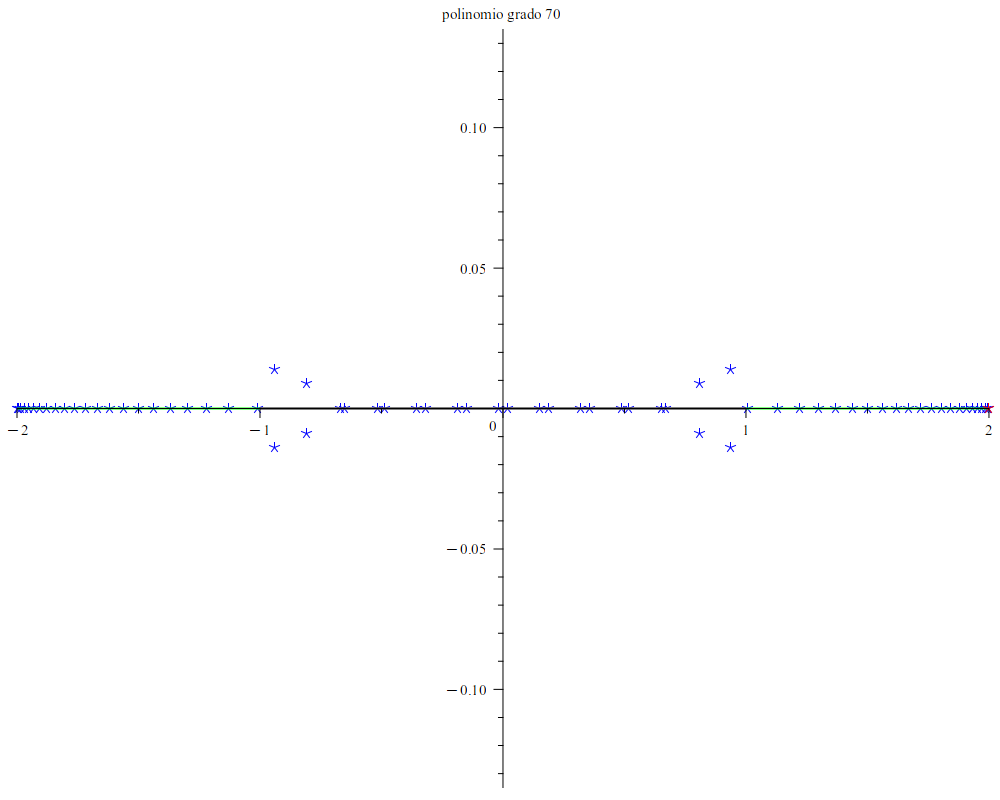
\includegraphics[width=\linewidth]{tfg_latex_etsiinf-2023.02.20/include/a-2b2c1d-1_zero.png}
			\caption*{\scriptsize Ceros $\varphi_{70}$}
		\end{subfigure}\hfill
		\begin{subfigure}[b]{0.4\columnwidth} % Modificado
			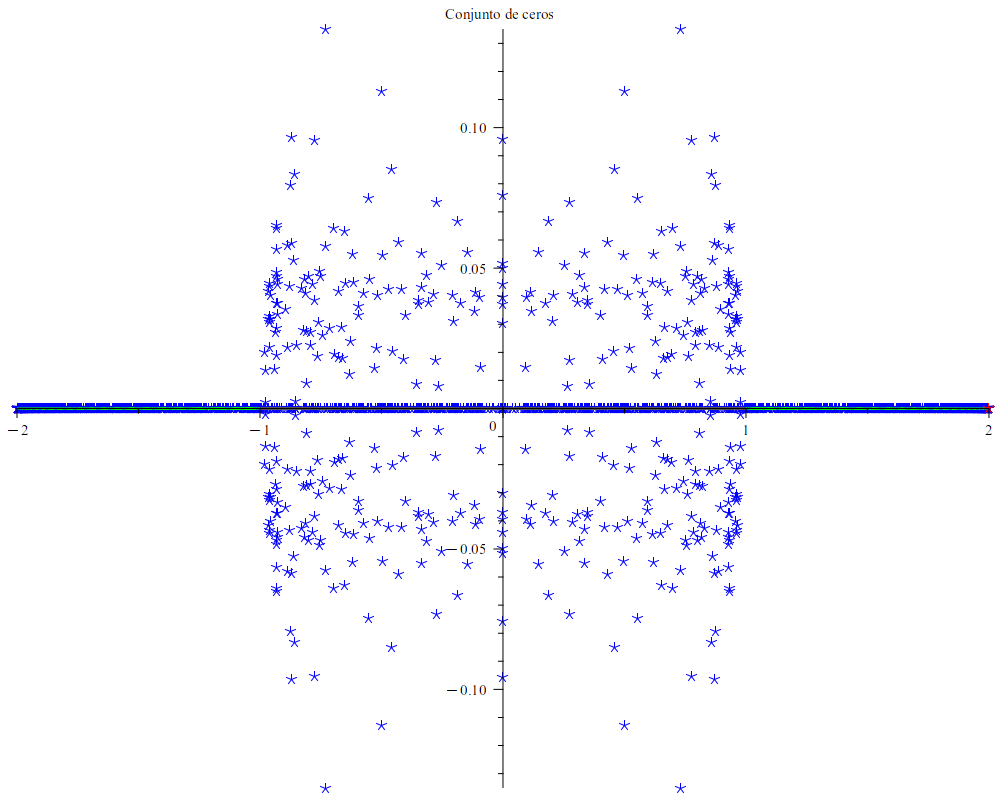
\includegraphics[width=\linewidth]{tfg_latex_etsiinf-2023.02.20/include/a-2b2c1d-1_zeros.png}
			\caption*{\scriptsize Ceros $\varphi_{0},\dots,\varphi_{70}$}
		\end{subfigure}
		\vspace{-0.5em} % Ajustado vspace, modificado de -0.3em
		\begin{subfigure}[b]{0.4\columnwidth} % Modificado
			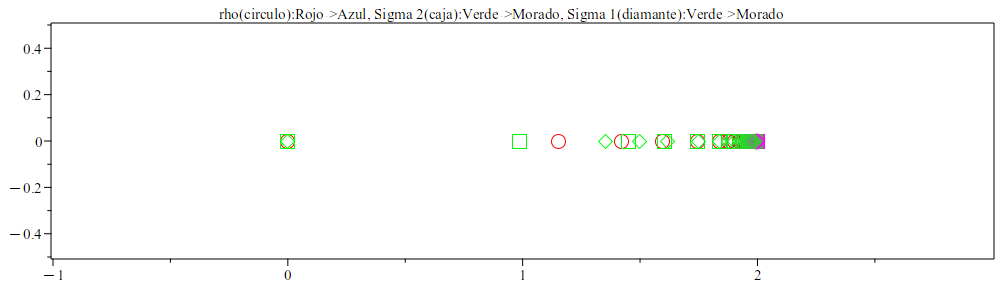
\includegraphics[width=\linewidth]{tfg_latex_etsiinf-2023.02.20/include/a-2b2c1d-1.png}
			\caption*{\scriptsize Sec. espectral}
		\end{subfigure}\hfill
		\begin{subfigure}[b]{0.4\columnwidth} % Modificado
			\tiny
			\textbf{Datos ($n=70$):}
			\begin{itemize}
				\item $\sigma_{1,70}=1.999$
				\item $\sigma_{2,70}=1.999$
				\item $R = 2$
				\item $\rho(\mathbf{D}_{70})=1.999$
				\item $\max\rho_k=1.999$
			\end{itemize}
		\end{subfigure}
	\end{figure}
	\vspace{-1em} % Ajustado vspace
\end{frame}

% --- DIAPOSITIVA 15B: CASO REAL - EJEMPLO SECUENCIALMENTE DOMINADO (OBSERVACIONES) ---
\begin{frame}{Caso Real: Ejemplo Secuencialmente Dominado - Observaciones}
	\begin{block}{Observaciones (Ej.1)} \small
		Caso secuencialmente dominado. $\mathcal{D}$ acotado. $\sigma_{1,n}, \sigma_{2,n}, \rho(\mathbf{D}_n) \to R=2$. Ceros en $[-2,2]$.
	\end{block}
\end{frame}

% --- DIAPOSITIVA 16A: CASO REAL - EJEMPLO SOPORTES DISJUNTOS ---
\begin{frame}{Caso Real: Ejemplo Soportes Disjuntos}
	\textbf{Ejemplo 2:}\;
	$\displaystyle
		\langle p, q \rangle_S
		= \int_{0}^{10} p(t)q(t) \, dt
		+ \int_{30}^{40} p'(t)q'(t) \, dt$
	\vspace{-0.8em}
	\begin{figure}
		\begin{subfigure}[b]{0.4\columnwidth} % Modificado
			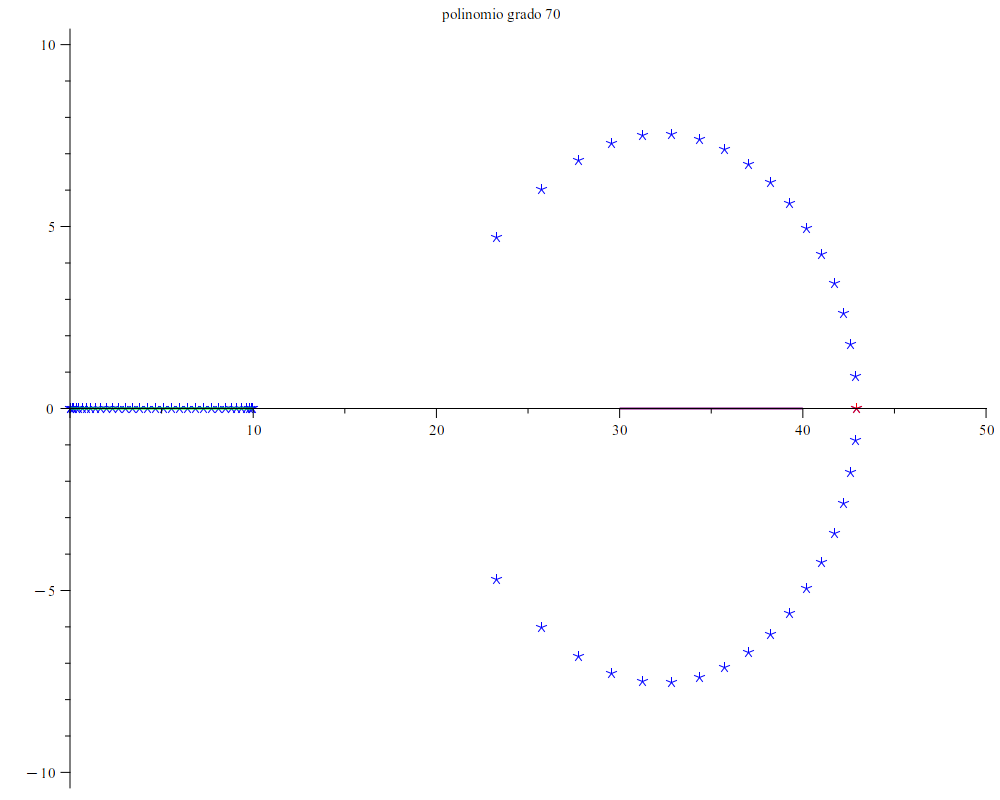
\includegraphics[width=\linewidth]{tfg_latex_etsiinf-2023.02.20/include/a0b10c30d40_zero.png}
			\caption*{\scriptsize Ceros $\varphi_{70}$}
		\end{subfigure}\hfill
		\begin{subfigure}[b]{0.4\columnwidth} % Modificado
			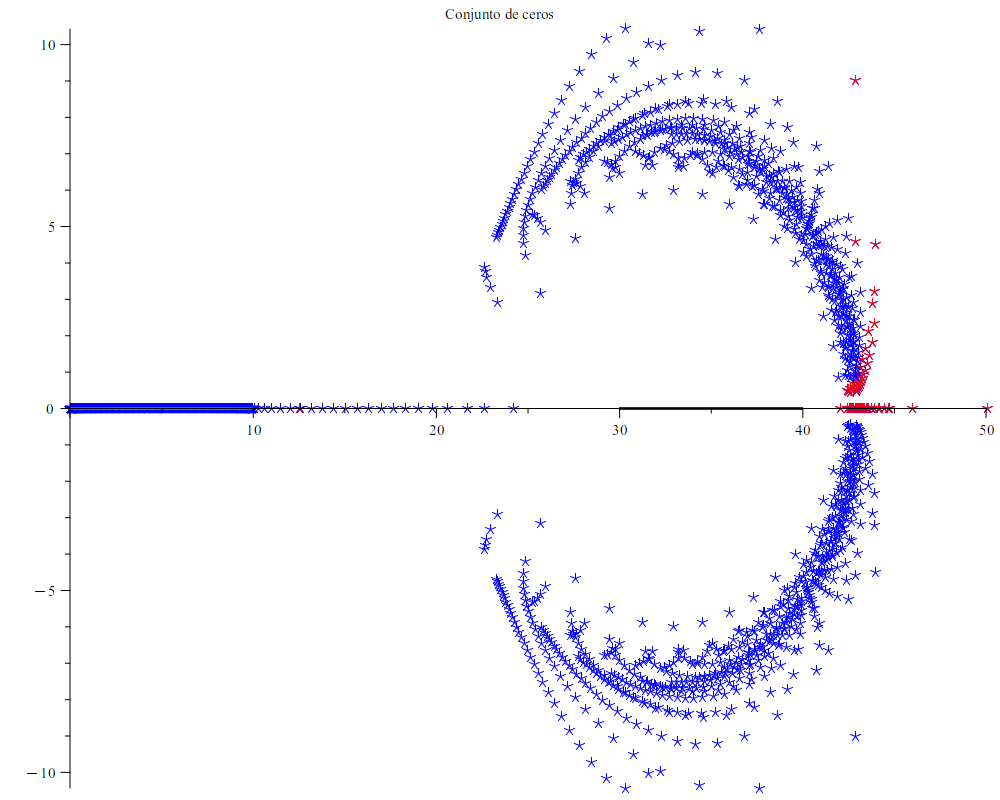
\includegraphics[width=\linewidth]{tfg_latex_etsiinf-2023.02.20/include/a0b10c30d40_zeros.png}
			\caption*{\scriptsize Ceros $\varphi_{0},\dots,\varphi_{70}$}
		\end{subfigure}
		\vspace{-0.5em} % Modificado de -0.3em
		\begin{subfigure}[b]{0.4\columnwidth} % Modificado
			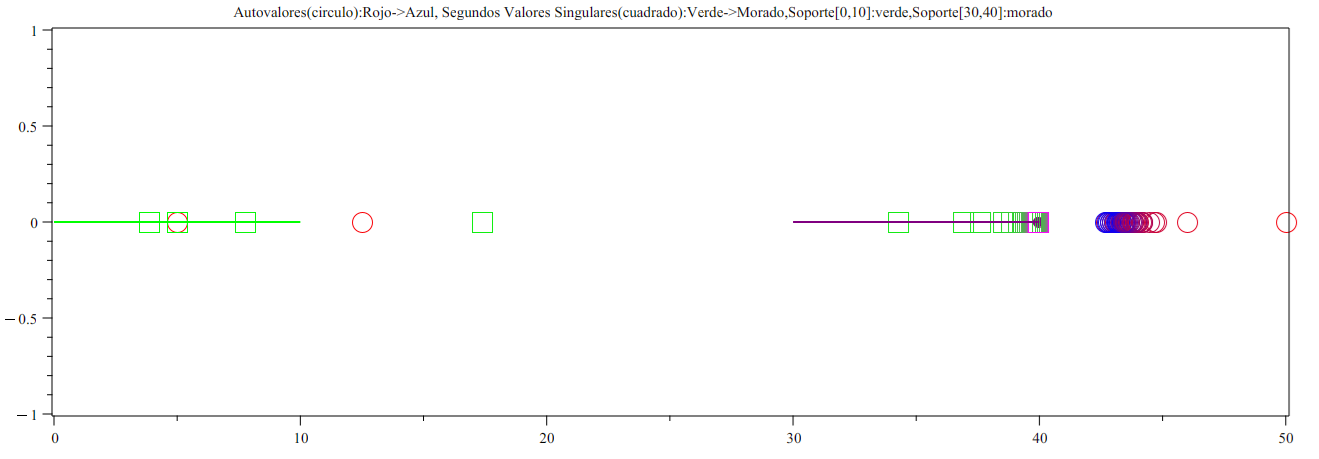
\includegraphics[width=\linewidth]{tfg_latex_etsiinf-2023.02.20/include/a0b10c30d40.png}
			\caption*{\scriptsize Sec. espectral}
		\end{subfigure}\hfill
		\begin{subfigure}[b]{0.4\columnwidth} % Modificado
			\tiny
			\textbf{Datos ($n=70$):}
			\begin{itemize}
				\item $\sigma_{1,70} \approx 9.27\text{e}16$
				\item $\sigma_{2,70} \approx 39.998$
				\item $R = 40$
				\item $\rho(\mathbf{D}_{70}) \approx 42.930$
				\item $\max\rho_k \approx 50.052$
			\end{itemize}
		\end{subfigure}
	\end{figure}
	\vspace{-1em}
\end{frame}

% --- DIAPOSITIVA 16A.1: CASO REAL - EJEMPLO SOPORTES DISJUNTOS (GRÁFICOS DE CEROS) ---
\begin{frame}{Caso Real: Ejemplo Soportes Disjuntos (Gráficos de Ceros)}
	\textbf{Ejemplo 2:}\;
	$\displaystyle
		\langle p, q \rangle_S
		= \int_{0}^{10} p(t)q(t) \, dt
		+ \int_{30}^{40} p'(t)q'(t) \, dt$
	\vspace{-0.8em}
	\begin{figure}
		\begin{subfigure}[b]{0.4\columnwidth} % Modificado
			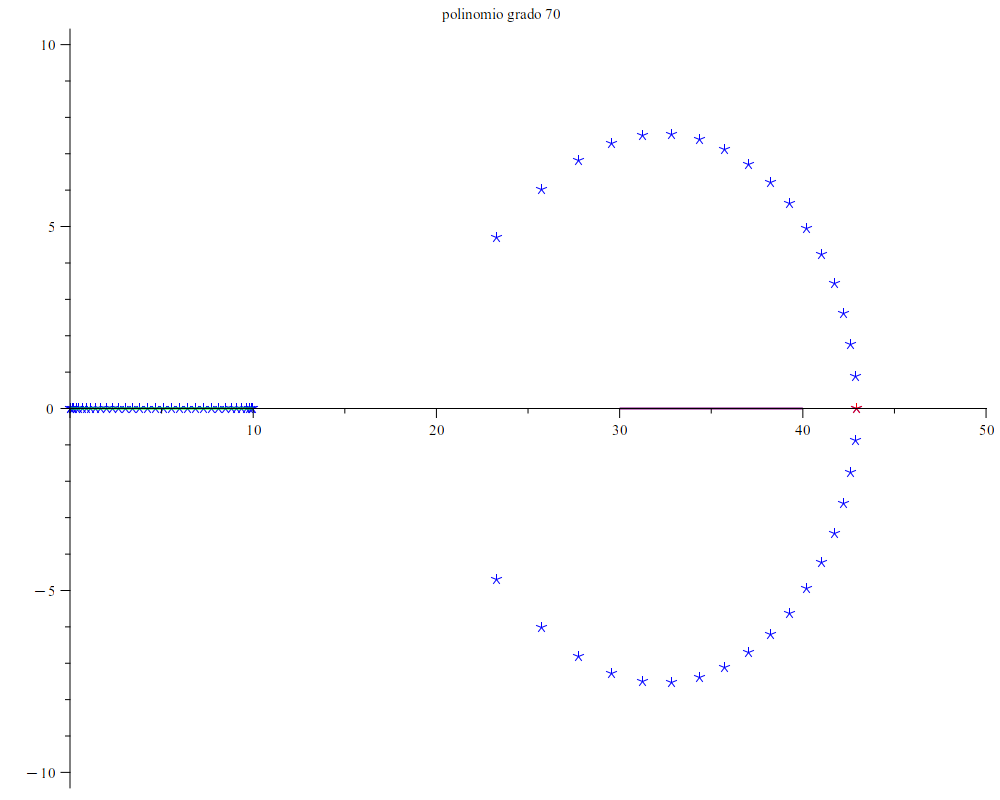
\includegraphics[width=\linewidth]{tfg_latex_etsiinf-2023.02.20/include/a0b10c30d40_zero.png}
			\caption*{\scriptsize Ceros $\varphi_{70}$}
		\end{subfigure}\hfill
		\begin{subfigure}[b]{0.4\columnwidth} % Modificado
			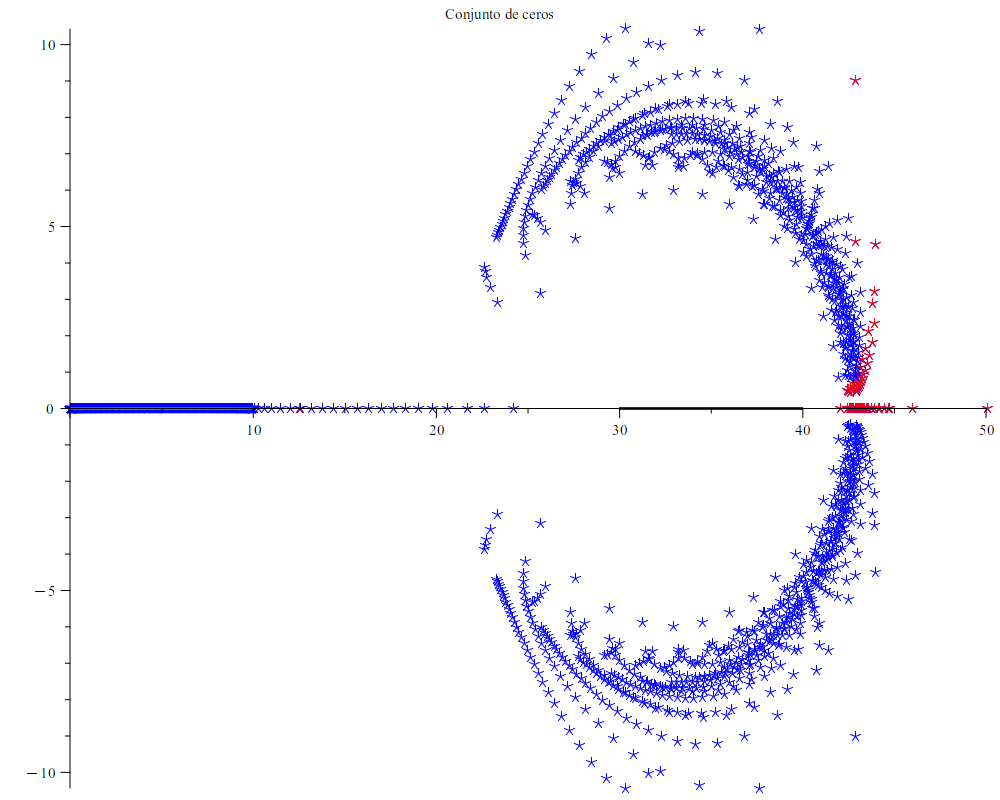
\includegraphics[width=\linewidth]{tfg_latex_etsiinf-2023.02.20/include/a0b10c30d40_zeros.png}
			\caption*{\scriptsize Ceros $\varphi_{0},\dots,\varphi_{70}$}
		\end{subfigure}
	\end{figure}
	\vspace{-1em}
\end{frame}

% --- DIAPOSITIVA 16A.2: CASO REAL - EJEMPLO SOPORTES DISJUNTOS (SECUENCIA ESPECTRAL Y DATOS) ---
\begin{frame}{Caso Real: Ejemplo Soportes Disjuntos (Secuencia Espectral y Datos)}
	\textbf{Ejemplo 2 (Continuación):}
	\vspace{0.5em} % Espacio para alinear con la fórmula si es necesario
	\begin{figure}
		\centering % Centrar las subfiguras restantes
		\begin{subfigure}[b]{0.4\columnwidth} % Modificado
			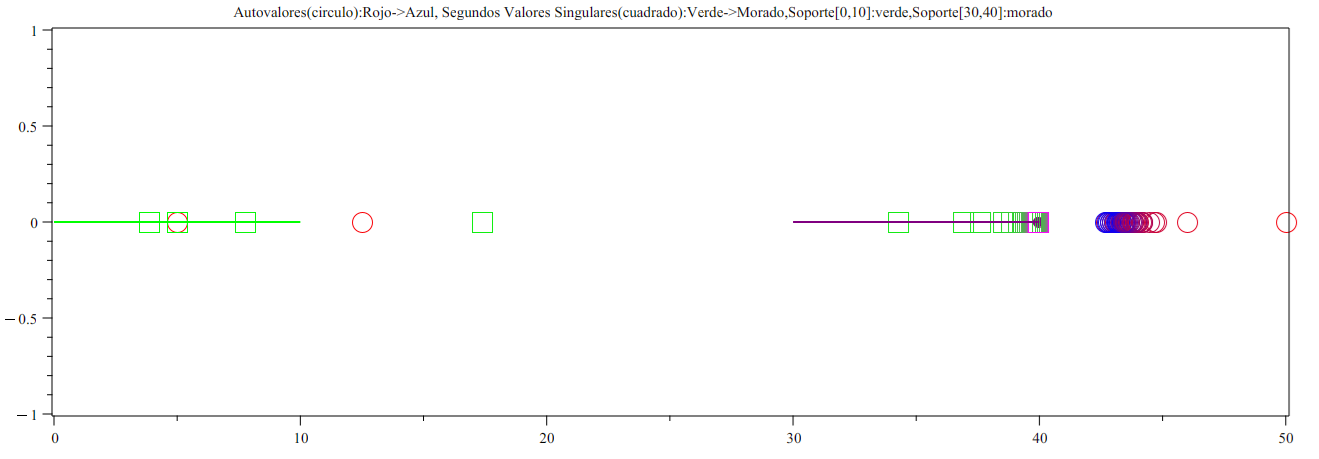
\includegraphics[width=\linewidth]{tfg_latex_etsiinf-2023.02.20/include/a0b10c30d40.png}
			\caption*{\scriptsize Sec. espectral}

		\end{subfigure}\hfill
		\begin{subfigure}[b]{0.4\columnwidth} % Modificado
			\tiny
			\textbf{Datos ($n=70$):}
			\begin{itemize}
				\item $\sigma_{1,70} \approx 9.27\text{e}16$
				\item $\sigma_{2,70} \approx 39.998$
				\item $R = 40$
				\item $\rho(\mathbf{D}_{70}) \approx 42.930$
				\item $\max\rho_k \approx 50.052$
			\end{itemize}
		\end{subfigure}
	\end{figure}
	\vspace{-1em}
\end{frame}

% --- DIAPOSITIVA 17A: CASO REAL - EJEMPLO ÁTOMO FUERA DEL SOPORTE ---
\begin{frame}{Caso Real: Átomo Fuera de $[-1,1]$}
	\textbf{Ejemplo 3:}\;
	$\displaystyle
		\langle p, q \rangle_S
		= \int_{-1}^{1} p(t) q(t) \, dt
		+ p'(2) q'(2)$
	\vspace{-0.8em}
	\begin{figure}
		\begin{subfigure}[b]{0.4\columnwidth} % Modificado
			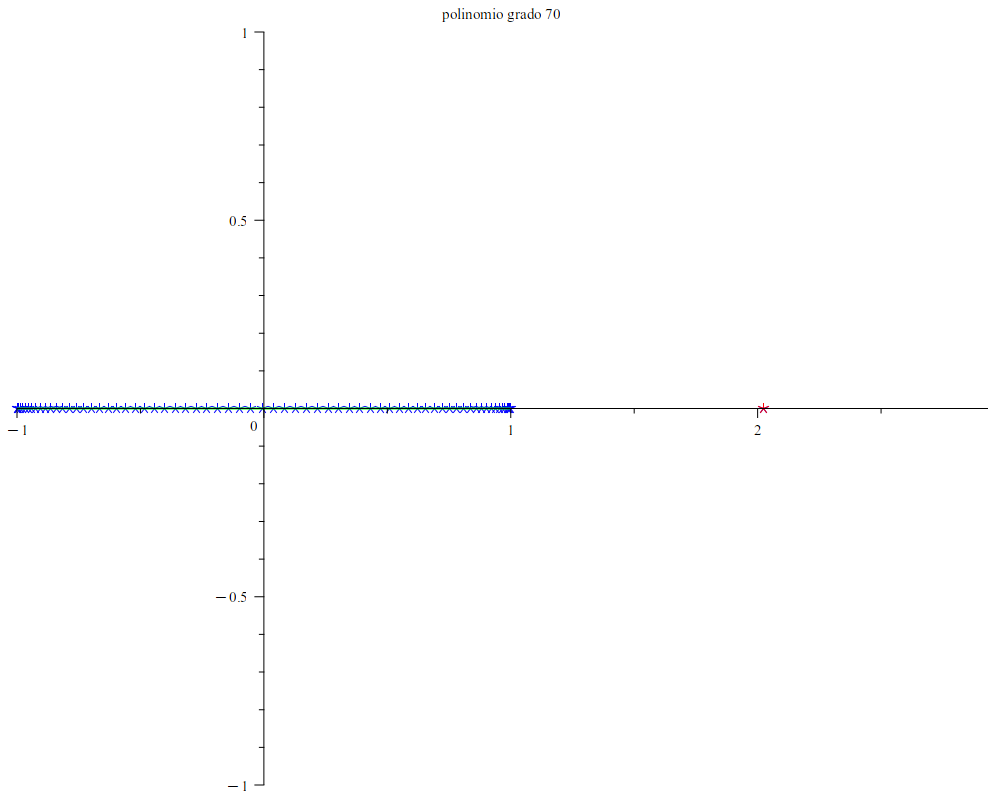
\includegraphics[width=\linewidth]{tfg_latex_etsiinf-2023.02.20/include/a-1b1t2_zero.png}
			\caption*{\scriptsize Ceros $\varphi_{70}$}
		\end{subfigure}\hfill
		\begin{subfigure}[b]{0.4\columnwidth} % Modificado
			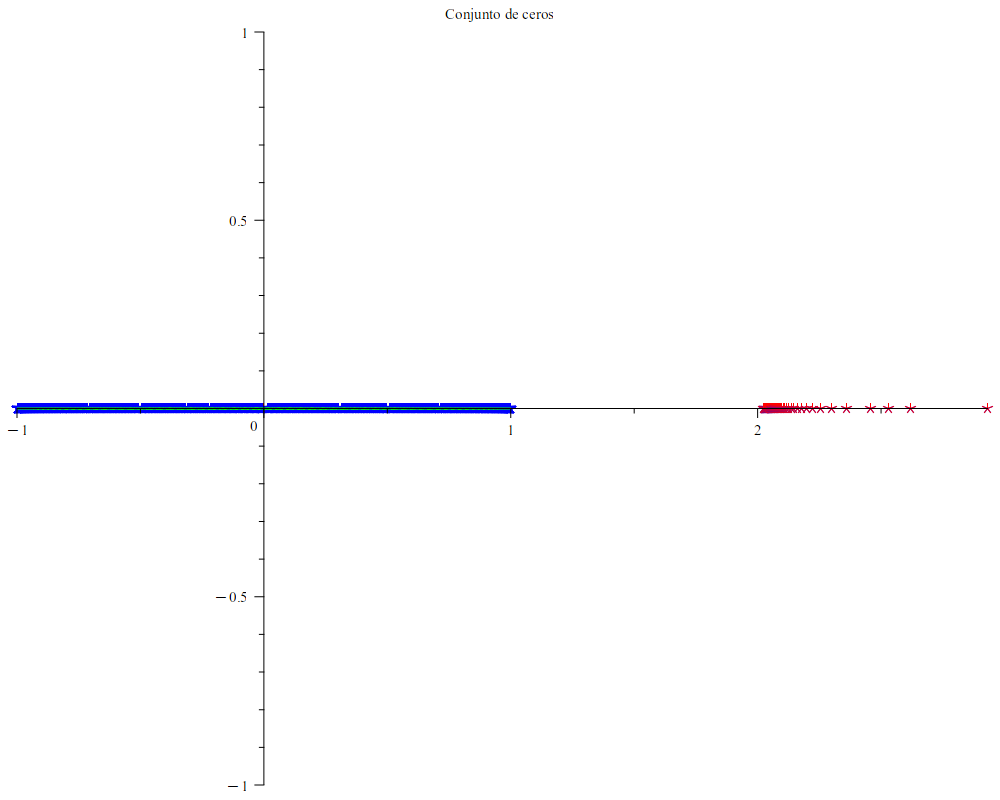
\includegraphics[width=\linewidth]{tfg_latex_etsiinf-2023.02.20/include/a-1b1t2_zeros.png}
			\caption*{\scriptsize Ceros $\varphi_{0},\dots,\varphi_{70}$}
		\end{subfigure}
		\vspace{-0.5em} % Modificado de -0.3em
		\begin{subfigure}[b]{0.4\columnwidth} % Modificado
			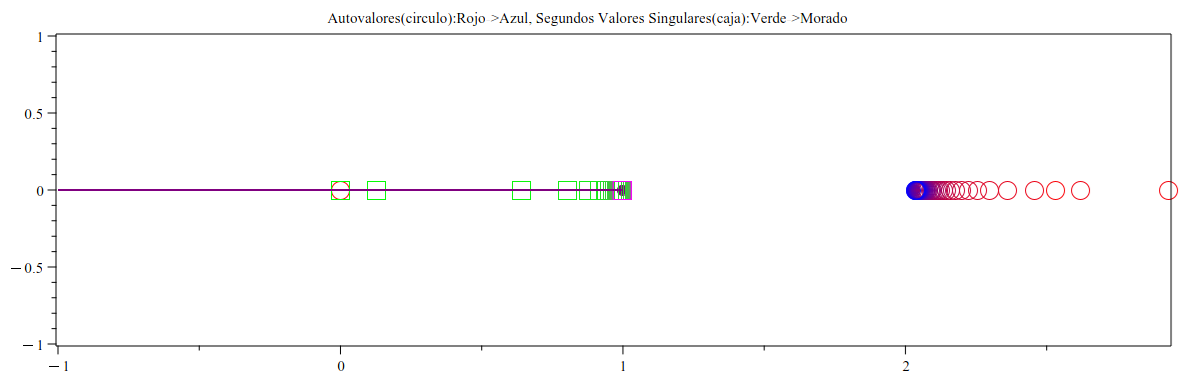
\includegraphics[width=\linewidth]{tfg_latex_etsiinf-2023.02.20/include/a-1b1t2.png}
			\caption*{\scriptsize Sec. espectral}
		\end{subfigure}\hfill
		\begin{subfigure}[b]{0.4\columnwidth} % Modificado
			\tiny
			\textbf{Datos ($n=70$):}
			\begin{itemize}
				\item $\sigma_{1,70} \approx 7.44\text{e}36$
				\item $\sigma_{2,70} \approx 0.999$
				\item $R = 2$ (átomo)
				\item $\rho(\mathbf{D}_{70}) \approx 2.025$
				\item $\max\rho_k \approx 2.933$
			\end{itemize}
		\end{subfigure}
	\end{figure}
	\vspace{-1em}
\end{frame}

% --- DIAPOSITIVA 17B: CASO REAL - EJEMPLO ÁTOMO FUERA (OBSERVACIONES) ---
\begin{frame}{Caso Real: Átomo Fuera de $[-1,1]$ - Observaciones}
	\begin{alertblock}{Observaciones (Ej.3)} \small
		Átomo $c=2$ fuera de $[-1,1]$. $\sigma_{1,n}$ diverge.
		$\rho(\mathbf{D}_n)$ acotado, influenciado por $c=2$.
		$\sigma_{2,n} \to \max_{[-1,1]}|z|=1$. Ceros atraídos por el átomo.
	\end{alertblock}
\end{frame}

% --- DIAPOSITIVA 18A: CASO CIRCUNFERENCIA - EJEMPLO SECUENCIALMENTE DOMINADO ---
\begin{frame}{Caso Circunferencia: Ejemplo Secuencialmente Dominado}
	\textbf{Ejemplo 4:}\;
	$\displaystyle
		\langle p, q \rangle_{S}=\int_{S_{1}(0)} p\overline{q}\, dm_{0;1} + \int_{S_{0.4}(0.4)} p'\overline{q'}\, dm_{0.4;0.4}$
	\vspace{-0.8em}
	\begin{figure}
		\begin{subfigure}[b]{0.4\columnwidth} % Modificado
			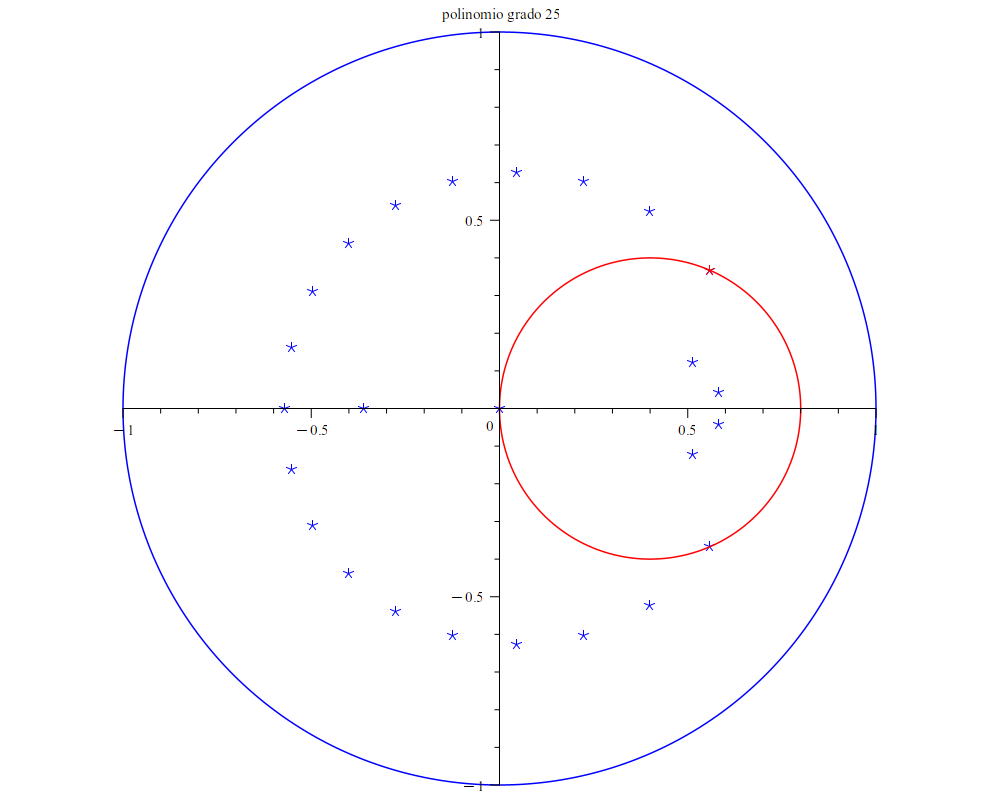
\includegraphics[width=\linewidth]{tfg_latex_etsiinf-2023.02.20/include/r1_1c1_0r2_0.4c2_0.4_zero.png}
			\caption*{\scriptsize Ceros $\varphi_{25}$}
		\end{subfigure}\hfill
		\begin{subfigure}[b]{0.4\columnwidth} % Modificado
			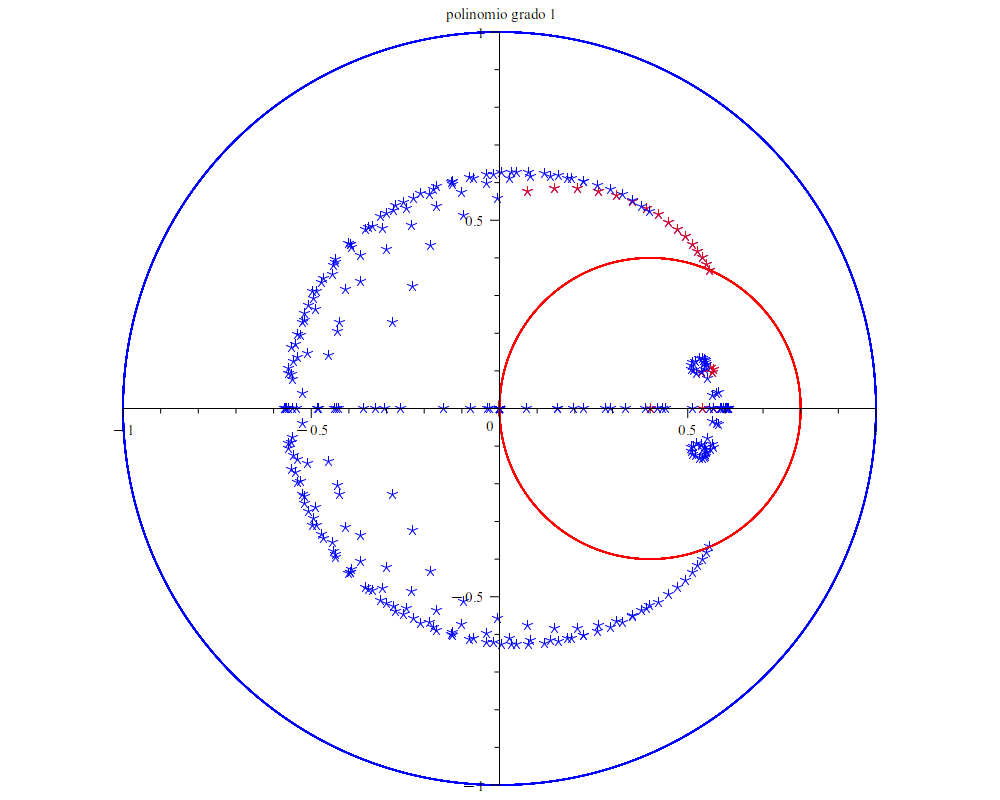
\includegraphics[width=\linewidth]{tfg_latex_etsiinf-2023.02.20/include/r1_1c1_0r2_0.4c2_0.4_zeros.png}
			\caption*{\scriptsize Ceros $\varphi_{0},\dots,\varphi_{25}$}
		\end{subfigure}
		\vspace{-0.5em} % Modificado de -0.3em
		\begin{subfigure}[b]{0.4\columnwidth} % Modificado
			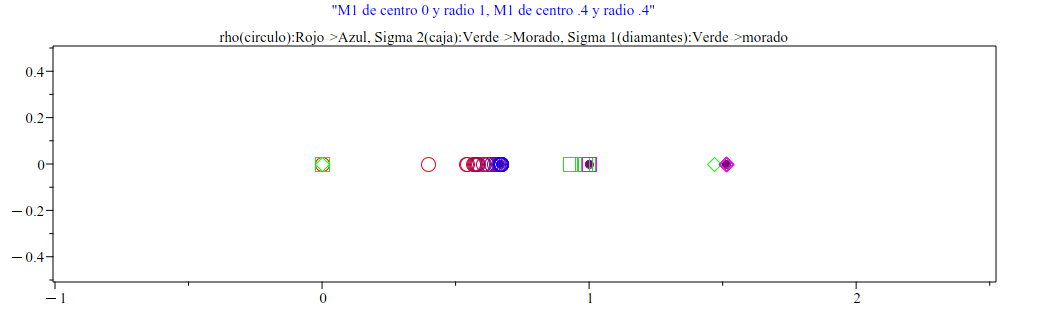
\includegraphics[width=\linewidth]{tfg_latex_etsiinf-2023.02.20/include/r1_1c1_0r2_0.4c2_0.4.png}
			\caption*{\scriptsize Sec. espectral}
		\end{subfigure}\hfill
		\begin{subfigure}[b]{0.4\columnwidth} % Modificado
			\tiny
			\textbf{Datos ($n=25$):}
			\begin{itemize}
				\item $\sigma_{1,25} \approx 1.516$
				\item $\sigma_{2,25} \approx 1.000$
				\item $R = 1$

				\item $\rho(\mathbf{D}_{25}) \approx 0.667$
				\item $\max\rho_k \approx 0.672$
			\end{itemize}
		\end{subfigure}
	\end{figure}
	\vspace{-1em}
\end{frame}

% --- DIAPOSITIVA 18B: CASO CIRCUNFERENCIA - EJEMPLO SEC. DOMINADO (OBSERVACIONES) ---
\begin{frame}{Caso Circunferencia: Ejemplo Secuencialmente Dominado - Observaciones}
	\begin{block}{Observaciones (Ej.4)} \small
		$S_{0.4}(0.4) \subset \mathbb{D}_1(0)$. $\mathcal{D}$ acotado. $\sigma_{1,n}$ converge.
		Ceros en $\mathbb{D}_1(0)$.
	\end{block}
\end{frame}

% --- DIAPOSITIVA 19A: CASO CIRCUNFERENCIA - EJEMPLO SOPORTES DISJUNTOS ---
\begin{frame}{Caso Circunferencia: Ejemplo Soportes Disjuntos}
	\textbf{Ejemplo 5:}\;
	$\displaystyle
		\langle p, q \rangle_{S}=\int_{S_{1}(0)} p\overline{q}\, dm_{0;1} + \int_{S_{1}(-10)} p'\overline{q'}\, dm_{-10;1}$
	\vspace{-0.8em}
	\begin{figure}
		\begin{subfigure}[b]{0.4\columnwidth} % Modificado
			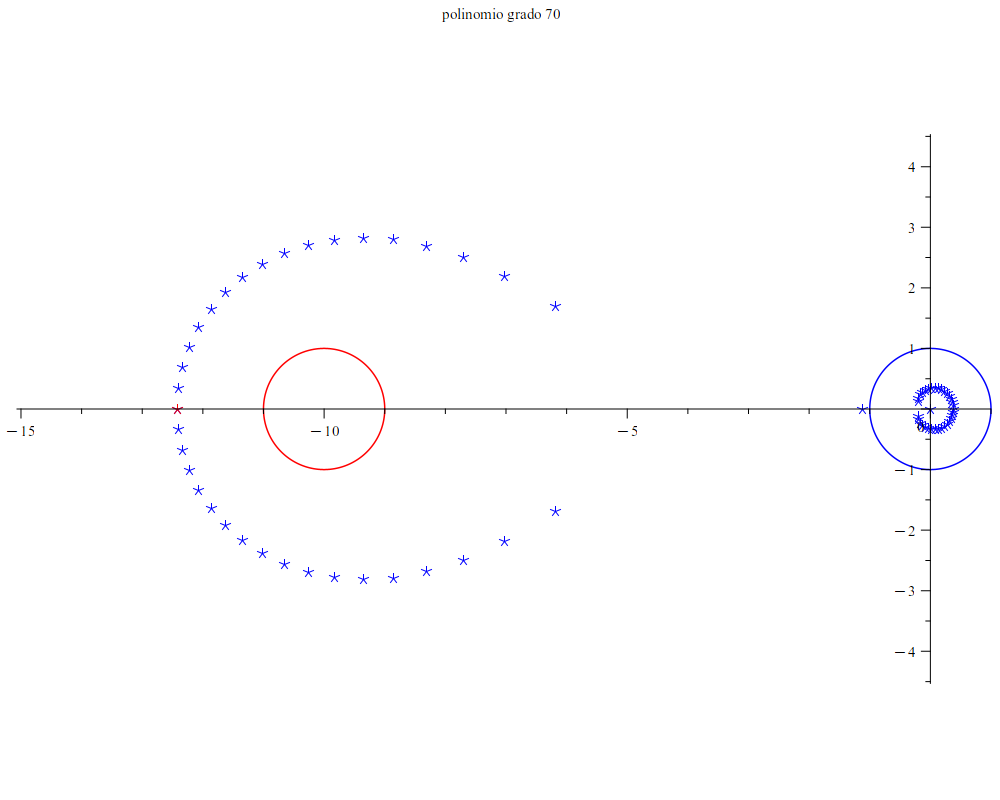
\includegraphics[width=\linewidth]{tfg_latex_etsiinf-2023.02.20/include/r1_1c1_0r2_1c2_-10_zero.png}
			\caption*{\scriptsize Ceros $\varphi_{70}$}
		\end{subfigure}\hfill
		\begin{subfigure}[b]{0.4\columnwidth} % Modificado
			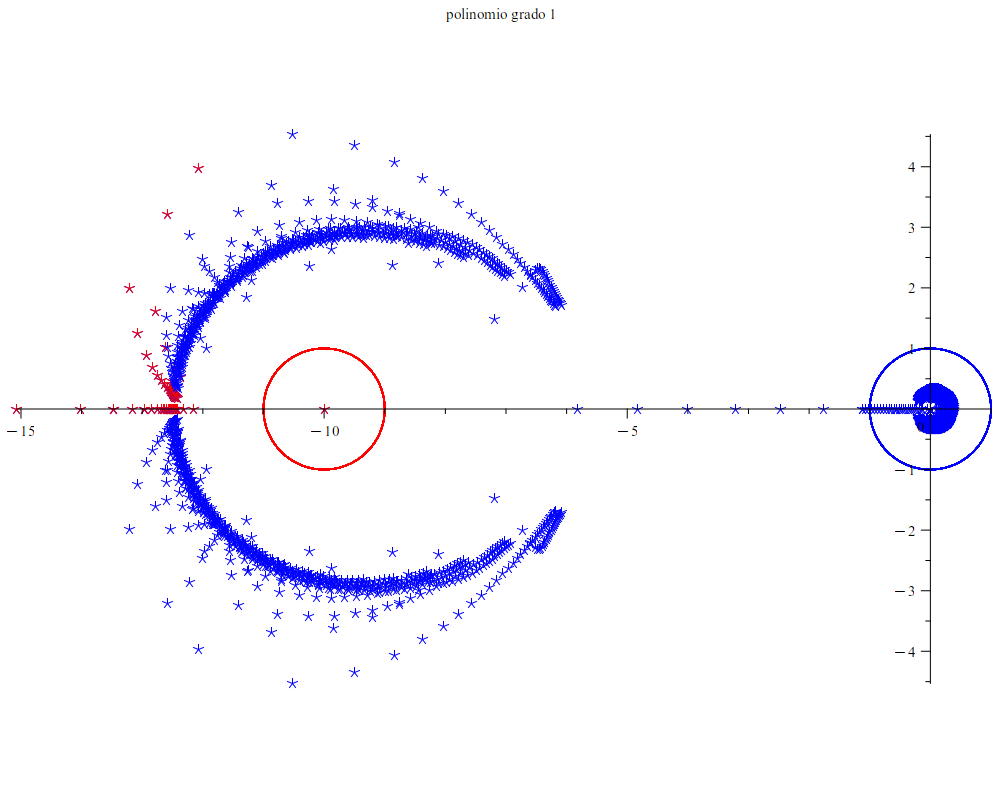
\includegraphics[width=\linewidth]{tfg_latex_etsiinf-2023.02.20/include/r1_1c1_0r2_1c2_-10_zeros.png}
			\caption*{\scriptsize Ceros $\varphi_{0},\dots,\varphi_{70}$}
		\end{subfigure}
		\vspace{-0.5em} % Modificado de -0.3em
		\begin{subfigure}[b]{0.4\columnwidth} % Modificado
			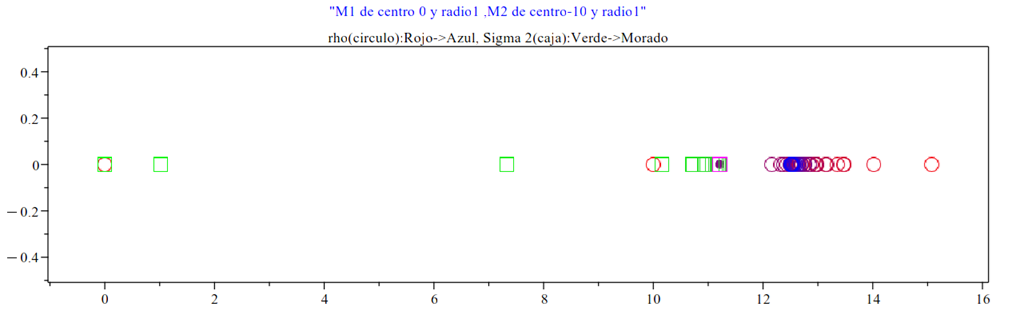
\includegraphics[width=\linewidth]{tfg_latex_etsiinf-2023.02.20/include/r1_1c1_0r2_1c2_-10.png}
			\caption*{\scriptsize Sec. espectral}
		\end{subfigure}\hfill
		\begin{subfigure}[b]{0.4\columnwidth} % Modificado
			\tiny
			\textbf{Datos ($n=70$):}
			\begin{itemize}
				\item $\sigma_{1,70} \approx 4.96\text{e}14$
				\item $\sigma_{2,70} \approx 11.211$
				\item $R = 11$
				\item $\rho(\mathbf{D}_{70}) \approx 12.424$
				\item $\max\rho_k \approx 15.074$
			\end{itemize}
		\end{subfigure}
	\end{figure}
	\vspace{-1em}
\end{frame}

% --- DIAPOSITIVA 19B: CASO CIRCUNFERENCIA - EJEMPLO SOP. DISJUNTOS (OBSERVACIONES) ---
\begin{frame}{Caso Circunferencia: Ejemplo Sop. Disjuntos - Observaciones}
	\begin{alertblock}{Observaciones (Ej.5)} \small
		Soportes disjuntos. $\sigma_{1,n}$ diverge.
		$\rho(\mathbf{D}_n)$ acotado. $\sigma_{2,n} \to R = 11$.
		Ceros pueden superar $R$.
	\end{alertblock}
\end{frame}

% --- DIAPOSITIVA 20A: CASO CIRCUNFERENCIA - EJEMPLO ÁTOMO FUERA ---
\begin{frame}{Caso Circunferencia: Ejemplo Átomo Fuera}
	\textbf{Ejemplo 6:}\;
	$\displaystyle
		\langle p, q \rangle_{S}=\int_{S_{1}(0)} p\overline{q}\, dm_{0;1} + p'(10)\overline{q'(10)}$
	\vspace{-0.8em}
	\begin{figure}
		\begin{subfigure}[b]{0.4\columnwidth} % Modificado
			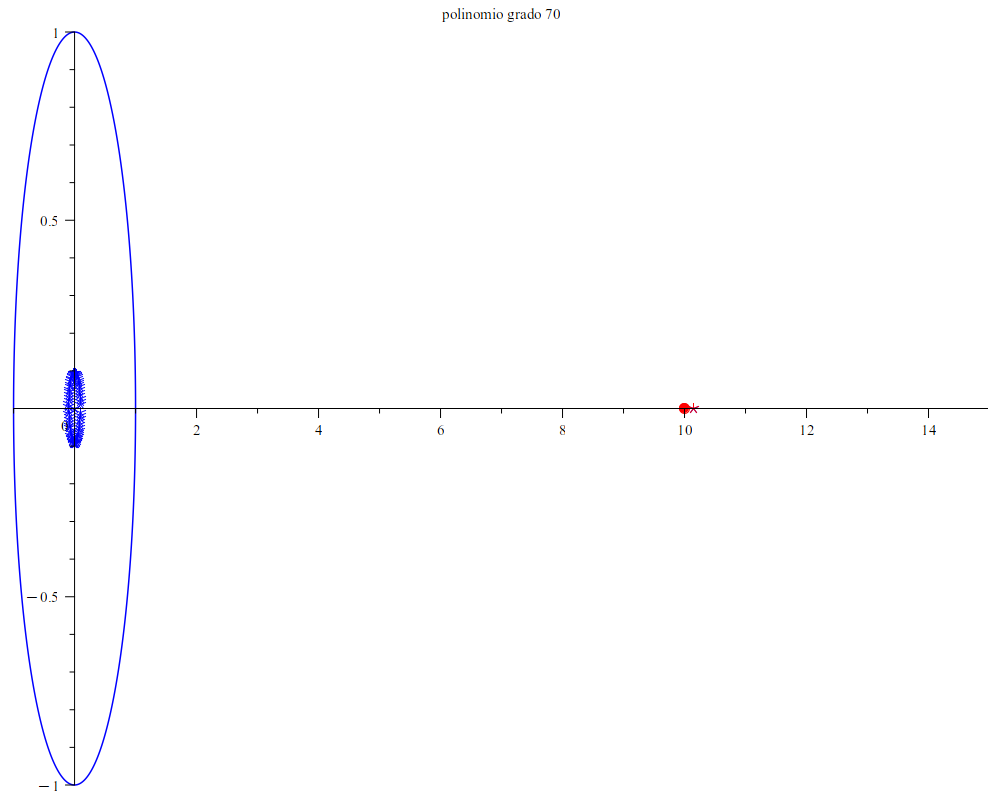
\includegraphics[width=\linewidth]{tfg_latex_etsiinf-2023.02.20/include/r1_1c1_0c2_10_zero.png}
			\caption*{\scriptsize Ceros $\varphi_{70}$}
		\end{subfigure}\hfill
		\begin{subfigure}[b]{0.4\columnwidth} % Modificado
			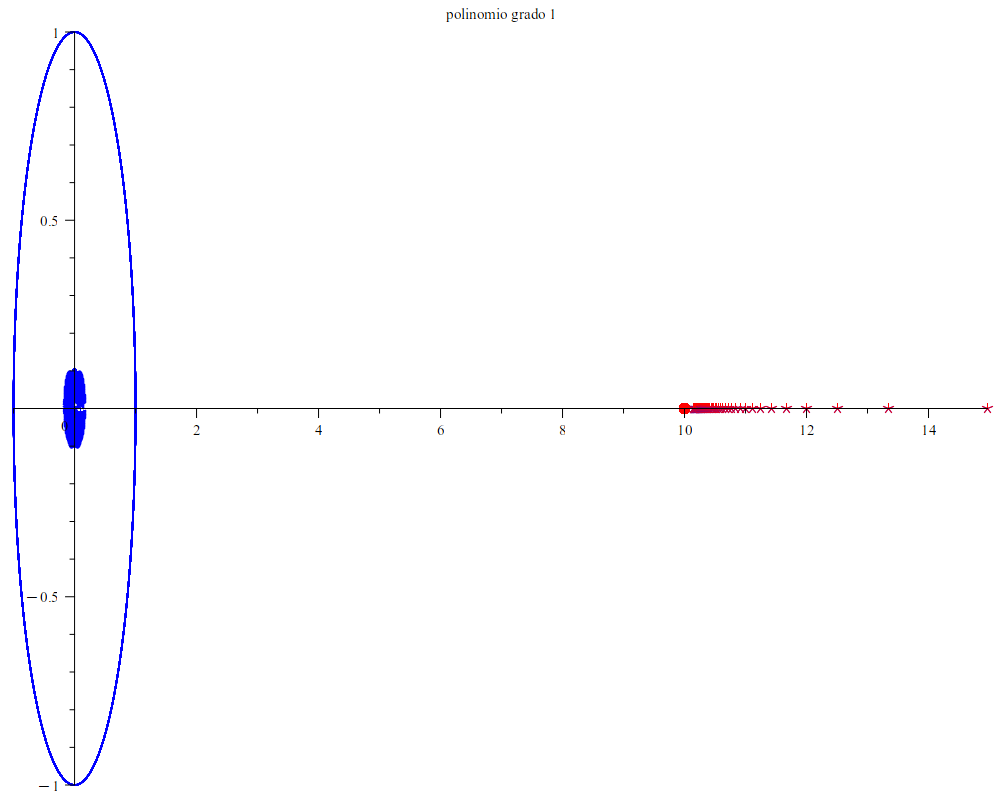
\includegraphics[width=\linewidth]{tfg_latex_etsiinf-2023.02.20/include/r1_1c1_0c2_10_zeros.png}
			\caption*{\scriptsize Ceros $\varphi_{0},\dots,\varphi_{70}$}
		\end{subfigure}
		\vspace{-0.5em} % Modificado de -0.3em
		\begin{subfigure}[b]{0.4\columnwidth} % Modificado
			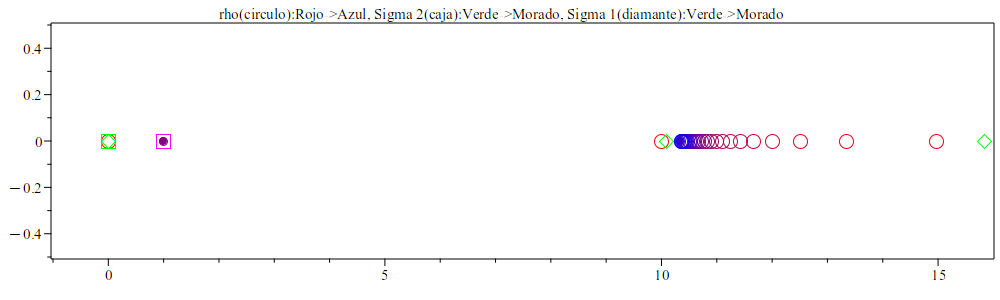
\includegraphics[width=\linewidth]{tfg_latex_etsiinf-2023.02.20/include/r1_1c1_0c2_10.png}
			\caption*{\scriptsize Sec. espectral}
		\end{subfigure}\hfill
		\begin{subfigure}[b]{0.4\columnwidth} % Modificado
			\tiny
			\textbf{Datos ($n=70$):}
			\begin{itemize}
				\item $\sigma_{1,70} \approx 3.50\text{e}26$
				\item $\sigma_{2,70} \approx 1.000$
				\item $R = 10$
				\item $\rho(\mathbf{D}_{70}) \approx 10.345$
				\item $\max\rho_k \approx 14.975$
			\end{itemize}
		\end{subfigure}
	\end{figure}
	\vspace{-1em}
\end{frame}

% --- DIAPOSITIVA 20B: CASO CIRCUNFERENCIA - EJEMPLO ÁTOMO FUERA (OBSERVACIONES) ---
\begin{frame}{Caso Circunferencia: Ejemplo Átomo Fuera - Observaciones}
	\begin{alertblock}{Observaciones (Ej.6)} \small
		Átomo $c=10$ fuera de $\mathbb{D}_1(0)$. $\sigma_{1,n}$ diverge.
		$\rho(\mathbf{D}_n)$ acotado, influenciado por $c=10$.
		$\sigma_{2,n} \to 1$. Ceros atraídos por el átomo.
	\end{alertblock}
\end{frame}

% --- DIAPOSITIVA 21A.1: ANÁLISIS Y CONJETURAS (IA) - OBSERVACIONES (SEC. DOMINADO) ---
\begin{frame}{Análisis y Conjeturas (Ia): Observaciones (Sec. Dominado)}
	\begin{block}{Caso Secuencialmente Dominado (Continuo Real)} \small
		El Cuadro 3.1 revela que en ejemplos secuencialmente dominados (e.g., Ej.1), donde $I_2=[c,d] \subset I_1=[a,b]$ y $w_1(t)/w_0(t)$ acotado en $I_1$:
		\begin{itemize}
			\item El operador multiplicación $\mathcal{D}$ es acotado.
			\item Los valores singulares $\sigma_{1,n}, \sigma_{2,n}$ y $\rho(\mathbf{D}_n)$ confirman la acotación.
			\item Los ceros están acotados por $\|\mathcal{D}\|$.
		\end{itemize}
	\end{block}
	\pause
	\begin{block}{Proposición (Caso Continuo Real)} \small
		Para $I_1=[a,b]$, $I_2=[c,d]$ con $[c,d] \subset [a,b]$, si definimos:
		$$R = \max\{|a|,|b|,|c|,|d|\}, \quad \alpha = \max_{t\in[a,b]}\frac{w_1(t)}{w_0(t)}$$
		Entonces $\mathcal{D}$ es acotado y $\|\mathcal{D}\| \le \sqrt{2(R^{2}+\alpha)}$.
	\end{block}
\end{frame}

% --- NUEVA DIAPOSITIVA: DEMOSTRACIÓN DE LA PROPOSICIÓN ---
\begin{frame}{Demostración: Operador Acotado (Caso Secuencialmente Dominado)}
	\begin{block}{Demostración} \tiny
		Sea $p(t)\in\mathbb{P}[t]$. Utilizando que $(a+b)^2\leq 2(a^2+b^2)$ para $a,b\ge0$:
		\begin{align}
			\|\mathcal{D}(p(t))\|^{2} & = \int_{a}^{b} t^2 p^2(t) w_0(t)\,dt + \int_{c}^{d} [(tp(t))']^2 w_1(t)\,dt                                            \\
			                          & = \int_{a}^{b} t^2 p^2(t) w_0(t)\,dt + \int_{c}^{d} [p(t)+tp'(t)]^2 w_1(t)\,dt                                         \\
			                          & \le \int_{a}^{b} t^2p^2(t)w_0(t)\, dt+2\left(\int_{c}^{d} p(t)^2w_1(t)\, dt +\int_{c}^{d} t^2p'(t)^2w_1(t)\, dt\right)
		\end{align}
	\end{block}
\end{frame}

% --- CONTINUACIÓN DE LA DEMOSTRACIÓN ---
\begin{frame}{Demostración: Operador Acotado (Continuación)}
	\begin{block}{Demostración (Continuación)} \tiny
		\begin{align}
			 & \le R^{2} \left(\int_{a}^{b} p^2(t)w_0(t)\, dt +  2\int_{c}^{d} p'(t)^2w_1(t)\, dt\right)+ 2\int_{c}^{d} p(t)^2w_1(t)\, dt \\
			 & \le 2R^{2} \|p(t)\|^{2} + 2\alpha \int_{c}^{d} p(t)^2w_0(t)\, dt                                                           \\
			 & \le 2R^{2} \|p(t)\|^{2} + 2\alpha \int_{a}^{b} p(t)^2w_0(t)\, dt                                                           \\
			 & = 2(R^{2}+\alpha)\|p(t)\|^{2}
		\end{align}
		Por tanto, $\|\mathcal{D}\| \le \sqrt{2(R^{2}+\alpha)}$. \qed
	\end{block}

	\begin{exampleblock}{Aplicación a los Ejemplos} \tiny
		\textbf{Ejemplo 1:} $I_1 = [-1,1]$ (con $w_0(t)=t^2$), $I_2 = [-1,1]$ (con $w_1(t)=t^{10}$).
		$R = 1$, $\alpha = 1$, entonces $\|\mathcal{D}\| \le \sqrt{4} = 2$.
		Consistente con $\sigma_{1,70} = 1.276 \le 2$.

		\textbf{Ejemplo 2:} $I_1 = [-2,2]$, $I_2 = [-1,1]$.
		$R = 2$, $\alpha = 1$, entonces $\|\mathcal{D}\| \le \sqrt{10} \approx 3.16$.
		Consistente con $\sigma_{1,70} = 1.999$.
	\end{exampleblock}
\end{frame}

% --- DIAPOSITIVA: CASOS NO SECUENCIALMENTE DOMINADOS ---
\begin{frame}{Análisis: Casos No Secuencialmente Dominados}
	\begin{alertblock}{Observaciones (Ejemplos 4-11)} \small
		Para casos con soportes disjuntos ($I_1 \cap I_2 = \emptyset$):
		\begin{itemize}
			\item $\sigma_{1,n}$ crece exponencialmente ($\approx 10^{16}$), sugiriendo $\mathcal{D}$ no acotado.
			\item $\sigma_{2,n}$ converge a $R = \max\{|a|,|b|,|c|,|d|\}$.
			\item $\rho(\mathbf{D}_n)$ permanece acotado, con comportamiento dependiente de la geometría:
			      \begin{itemize}
				      \item Si $I_1$ contiene el extremo de mayor módulo: $\rho(\mathbf{D}_n) \to R$.
				      \item Si $I_2$ contiene el extremo de mayor módulo: $\rho(\mathbf{D}_n) \to R + k$ con $k \geq 0$.
			      \end{itemize}
		\end{itemize}
	\end{alertblock}
\end{frame}

% --- DIAPOSITIVA: CASOS CON ÁTOMO ---
\begin{frame}{Análisis: Casos con Átomo}
	\begin{alertblock}{Observaciones (Ejemplos 12-15)} \small
		Para productos $\langle p,q \rangle = \int_{a}^{b} pq \, dt + p'(c)q'(c)$:
		\begin{itemize}
			\item $\sigma_{1,n}$ extremadamente grande ($\approx 10^{36}$), indicando $\mathcal{D}$ no acotado.
			\item $\sigma_{2,n}$ converge a $R_0 = \max\{|a|,|b|\}$ (radio del soporte integral).
			\item Comportamiento de $\rho(\mathbf{D}_n)$ depende de la posición del átomo:
			      \begin{itemize}
				      \item Si $c \in [a,b]$: $\rho(\mathbf{D}_n) \to R_0$.
				      \item Si $c \notin [a,b]$: $\rho(\mathbf{D}_n)$ influenciado por $|c|$, ceros atraídos hacia $c$.
			      \end{itemize}
		\end{itemize}
	\end{alertblock}
\end{frame}

% --- DIAPOSITIVA: CASO CIRCUNFERENCIA - ANÁLISIS ---
\begin{frame}{Análisis: Caso Circunferencia}
	\begin{block}{Clasificación por Contención} \small
		Para productos $\langle p,q \rangle = \int_{S_{r_b}(b)} p\overline{q} \, dm + \int_{S_{r_a}(a)} p'\overline{q'} \, dm$:
		\begin{enumerate}
			\item \textbf{$S_{r_a}(a) \subset \mathbb{D}_{r_b}(b)$}: Caso secuencialmente dominado, $\mathcal{D}$ acotado.
			\item \textbf{$a \in \mathbb{D}_{r_b}(b)$ pero $S_{r_a}(a) \not\subset \mathbb{D}_{r_b}(b)$}: $\mathcal{D}$ acotado.
			\item \textbf{$a \notin \mathbb{D}_{r_b}(b)$}: Comportamiento de $\mathcal{D}$ incierto, evidencia sugiere no acotación.
		\end{enumerate}
	\end{block}
	\pause
	\begin{block}{Casos con Átomo Complejo} \small
		\begin{itemize}
			\item Si $c \in \mathbb{D}_{r_b}(b)$: $\mathcal{D}$ acotado (casos secuencialmente dominados).
			\item Si $c \notin \mathbb{D}_{r_b}(b)$: Evidencia sugiere $\mathcal{D}$ no acotado.
		\end{itemize}
	\end{block}
\end{frame}

% --- DIAPOSITIVA 21B: ANÁLISIS Y CONJETURAS (IB) - OBSERVACIONES CLAVE ---
\begin{frame}{Análisis y Conjeturas (Ib): Observación Fundamental}
	\begin{alertblock}{Observación Crucial (Todos los Ejemplos)} \small
		En la totalidad de los ejemplos numéricos (Cuadros 3.1 y 3.2):
		\begin{itemize}
			\item \textbf{Acotación Universal del Radio Espectral}: Incluso cuando $\mathcal{D}$ no es acotado ($\sigma_{1,n} \to \infty$), el radio espectral $\rho(\mathbf{D}_n)$ permanece acotado.
			\item \textbf{Convergencia del Segundo Valor Singular}: $\sigma_{2,n}$ converge consistentemente:
			      \begin{itemize}
				      \item En casos continuos: a $R = \max\{|z| : z \in \text{supp}(\mu_1) \cup \text{supp}(\mu_2)\}$.
				      \item En casos con átomo: a $R_0 = \max\{|z| : z \in \text{supp}(\mu_1)\}$.
			      \end{itemize}
		\end{itemize}
	\end{alertblock}
\end{frame}

% --- DIAPOSITIVA: SOPORTE TEÓRICO ---
\begin{frame}{Soporte Teórico: Teoremas de Entrelazamiento}
	\begin{block}{Teorema de Entrelazamiento de Cauchy} \small
		Sea $A$ matriz de orden $n$ y $B$ submatriz principal de orden $n-1$. Si $\lambda_n \leq \cdots \leq \lambda_1$ son autovalores de $A$ y $\mu_{n-1} \leq \cdots \leq \mu_1$ de $B$:
		$$\lambda_n \leq \mu_{n-1} \leq \cdots \leq \mu_2 \leq \lambda_1$$
	\end{block}
	\pause
	\begin{block}{Aplicación a Matrices de Hessenberg} \small
		Para matrices infinitas de Hessenberg $\mathbf{D}$ con secciones $\mathbf{D}_n$:
		\begin{itemize}
			\item La sucesión $\{\sigma_{2,n}\}$ es creciente.
			\item Existe $\lim_{n \to \infty} \sigma_{2,n} \leq \infty$.
		\end{itemize}
	\end{block}
\end{frame}

% --- DIAPOSITIVA 22A.1: CONJETURAS PRINCIPALES (IIA) - CONJETURA 1 (ACOTACIÓN) ---
\begin{frame}{Conjetura 1: Acotación Universal del Radio Espectral}
	\begin{block}{Conjetura Principal} \small
		Basándose en la evidencia numérica exhaustiva de los Cuadros 3.1 y 3.2:
		$$\lim_{n \to \infty} \rho(\mathbf{D}_n) < \infty$$
		Esta propiedad se mantiene incluso cuando el operador $\mathcal{D}$ no es acotado.
	\end{block}
	\pause
	\begin{block}{Comportamiento Asintótico} \small
		El radio espectral tiende a converger a $R + k$, donde:
		\begin{itemize}
			\item $R = \max\{|z| : z \in \text{supp}(\mu_1) \cup \text{supp}(\mu_2)\}$
			\item $k \in \mathbb{R}$ depende de la geometría relativa de los soportes
			\item $k \geq 0$ cuando el soporte de la derivada contiene el extremo de mayor módulo
		\end{itemize}
	\end{block}
\end{frame}

% --- DIAPOSITIVA 22b: CONJETURAS PRINCIPALES (IIIB) - FORMULACIÓN ---
\begin{frame}{Conjetura 2: Convergencia del Segundo Valor Singular}
	\begin{block}{Conjetura 2} \small
		El segundo mayor valor singular $\sigma_{2,n}$ de $\mathbf{D}_n$ converge:
		$$\lim_{n \to \infty} \sigma_{2,n} < \infty$$
		Específicamente:
		\begin{itemize}
			\item En casos continuos: converge a $R = \max\{|z| : z \in \text{supp}(\mu_1) \cup \text{supp}(\mu_2)\}$
			\item En casos con átomo: converge a $R_0 = \max\{|z| : z \in \text{supp}(\mu_1)\}$
		\end{itemize}
	\end{block}
	\pause
	\begin{exampleblock}{Soporte Teórico} \small
		Resultados parciales apoyan estas conjeturas:
		\begin{itemize}
			\item Teorema de entrelazamiento de Cauchy
			\item Propiedades de matrices de Hessenberg
			\item Análisis de valores singulares \cite{singularValuesOfHessenbergMatrices}
		\end{itemize}
	\end{exampleblock}
\end{frame}

% --- DIAPOSITIVA 23A.1: ANÁLISIS Y CONJETURAS (IIIA) - TRASLACIONES (OBSERVACIÓN Y CONJETURA) ---
\begin{frame}{Conjetura 3: Traslaciones de Soportes}
	\begin{block}{Observación Empírica} \small
		Cuando los soportes en $\mathbb{R}$ se trasladan a lo largo del eje real, los ceros se trasladan de manera correspondiente.
	\end{block}
	\pause
	\begin{block}{Conjetura 3} \small
		Los ceros de polinomios ortogonales de Sobolev asociados a medidas trasladadas en el eje real se trasladan mediante la misma traslación.
	\end{block}
	\pause
	\begin{alertblock}{Limitaciones} \small
		Si la traslación tiene componente imaginaria, pueden ocurrir comportamientos anómalos que requieren investigación adicional.
	\end{alertblock}
\end{frame}

% --- DIAPOSITIVA 23B: ANÁLISIS Y CONJETURAS (IIIB) - SEMEJANZA ---
\begin{frame}{Transformaciones de Semejanza: Limitaciones en Sobolev}
	\begin{block}{Caso Estándar (Una Medida)} \small
		Si $f(z) = \alpha z + \beta$ es una semejanza, los ceros de $P_n(z)$ se transforman mediante $f$ a los ceros de $P_n^f(z)$.
	\end{block}
	\pause
	\begin{alertblock}{Precaución en Productos de Sobolev} \small
		En productos de Sobolev, la aplicabilidad directa de este resultado \textbf{no es general}:
		\begin{itemize}
			\item Ejemplos con traslaciones complejas muestran comportamientos anómalos
			\item La teoría clásica de transformaciones no se extiende automáticamente
			\item Se requiere investigación específica para productos de Sobolev
		\end{itemize}
	\end{alertblock}
\end{frame}

% --- DIAPOSITIVA FINAL: RESUMEN DE CONJETURAS ---
\begin{frame}{Resumen: Conjeturas Principales}
	\begin{block}{Tres Conjeturas Fundamentales} \small
		\begin{enumerate}
			\item \textbf{Acotación Universal}: $\lim_{n \to \infty} \rho(\mathbf{D}_n) < \infty$ incluso cuando $\mathcal{D}$ no es acotado.
			\item \textbf{Convergencia $\sigma_2$}: $\lim_{n \to \infty} \sigma_{2,n} = R$ (casos continuos) o $R_0$ (casos atómicos).
			\item \textbf{Invarianza por Traslación}: Los ceros se trasladan con traslaciones reales de los soportes.
		\end{enumerate}
	\end{block}
	\pause
	\begin{exampleblock}{Implicaciones} \small
		Estas conjeturas establecen:
		\begin{itemize}
			\item Cotas universales para ceros de polinomios de Sobolev
			\item Criterios predictivos basados en la geometría de soportes
			\item Fundamentos para futuras demostraciones rigurosas
		\end{itemize}
	\end{exampleblock}
\end{frame}
% --- CORRESPONDE A: conclusiones.tex ---
% --- DIAPOSITIVA 25: CONCLUSIONES (II) - PRINCIPALES LOGROS ---
\begin{frame}{Conclusiones: Principales Logros}
	\footnotesize
	\begin{itemize}
		\item Estudio del marco teórico matricial para Polinomios Ortogonales de Sobolev.
		\item Validación numérica de condiciones de acotación de $\mathcal{D}$ en diversos contextos geométricos.
		\item Análisis pionero del comportamiento de $\sigma_{2,n}$ en operadores no secuencialmente dominados.
		\item Implementación de algoritmos eficientes en \textsc{Maple}.
		\item Creación de un sistema interactivo de visualización.
		\item Desarrollo personal.
	\end{itemize}
\end{frame}

% --- CORRESPONDE A: conclusiones.tex ---
% --- DIAPOSITIVA 28: LÍNEAS DE TRABAJO FUTURO (I) ---
\begin{frame}{Líneas de Trabajo Futuro (I)}
	\footnotesize
	Se abren diversos frentes de investigación:
	\begin{itemize}
		\item \textbf{Productos Sobolev de orden superior ($N>1$):}
		      \begin{itemize}
			      \item Incorporar derivadas de segundo y tercer orden.
			      \item Analizar valores singulares siguientes ($\sigma_{3,n}, \sigma_{4,n},...$).
		      \end{itemize}
		      \pause
		\item \textbf{Leyes de distribución de ceros:}
		      \begin{itemize}
			      \item Derivar distribuciones límite (tipo medida de equilibrio) para los ceros en distintos regímenes (analogía con Ullman-Stahl).
		      \end{itemize}
		      \pause
		\item \textbf{Convergencia del autovalor máximo:}
		      \begin{itemize}
			      \item Investigar si el autovalor que determina $\rho(\mathbf{D}_n)$ converge.
		      \end{itemize}
	\end{itemize}
\end{frame}

% --- DIAPOSITIVA 30: LÍNEAS DE TRABAJO FUTURO (III) - EJEMPLOS CON DERIVADAS DE ORDEN SUPERIOR ---
\begin{frame}{Líneas de Trabajo Futuro (II) - Ejemplos con Derivadas de Orden Superior}
	\footnotesize
	\begin{columns}[T]
		\begin{column}{0.48\textwidth}
			\textbf{Ejemplo 1:}
			\tiny
			$\langle p,q \rangle_{S}=\int_{0}^{10} pq\, dt + \int_{30}^{40} p'q' \, dt + \int_{60}^{70} p''q'' \, dt$

			\vspace{-0.3em}
			\begin{figure}
				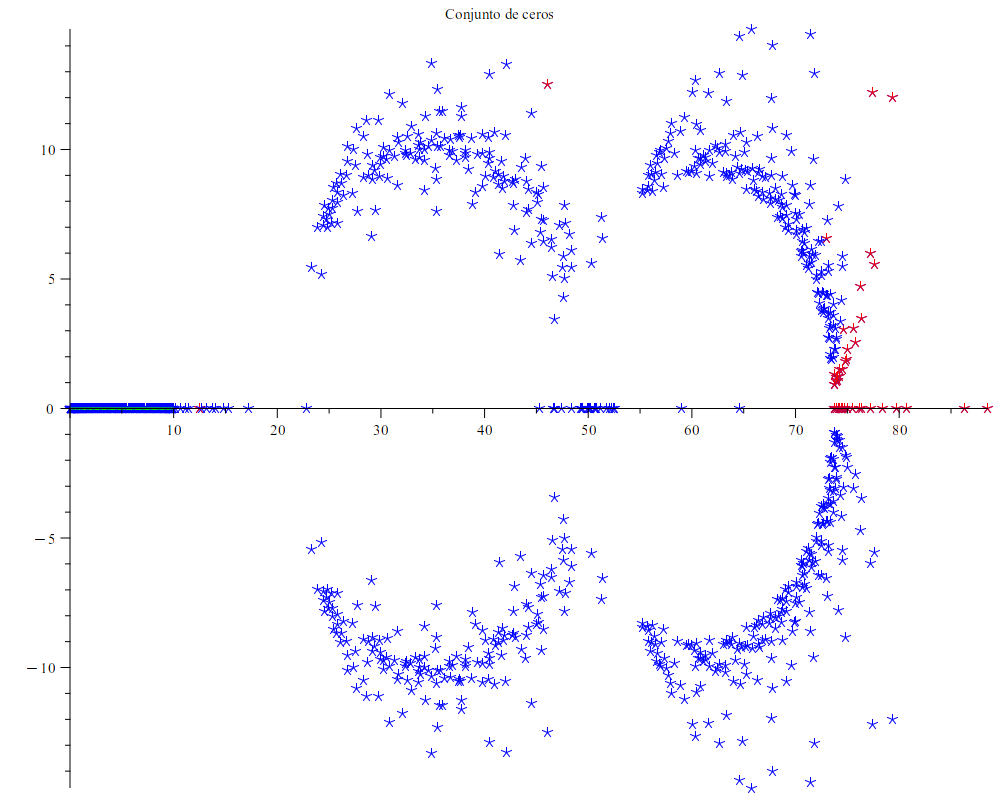
\includegraphics[width=0.8\linewidth]{tfg_latex_etsiinf-2023.02.20/include/a0b10c30d40e60f70_zeros.png}
			\end{figure}
			\vspace{-1.5em}

			\textbf{Datos ($n=70$):}
			\begin{itemize}
				\item $\sigma_{1,70} \approx 4.94 \times 10^{8}$
				\item $\sigma_{2,70} \approx 1.85 \times 10^{8}$
				\item $\sigma_{3,70} \approx 69.956$
				\item $R = 70$
				\item $\rho(\mathbf{D}_{70}) \approx 73.791$
			\end{itemize}
		\end{column}

		\begin{column}{0.48\textwidth}
			\textbf{Ejemplo 2:}
			\tiny
			$\langle p,q \rangle_{S}=\int_{0}^{10} pq\, dt + \int_{30}^{40} p'q' \, dt + p''(0)q''(0)$

			\vspace{-0.3em}
			\begin{figure}
				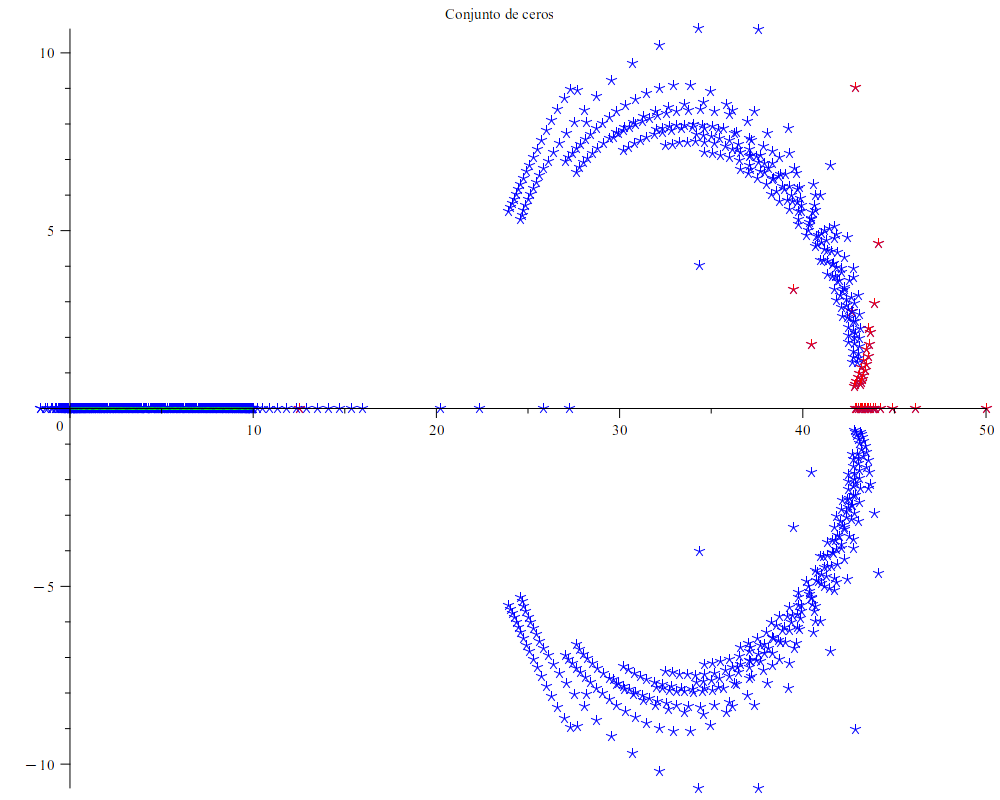
\includegraphics[width=0.8\linewidth]{tfg_latex_etsiinf-2023.02.20/include/a0b10c30d40t0_zeros.png}
			\end{figure}
			\vspace{-1.5em}

			\textbf{Datos ($n=70$):}
			\begin{itemize}
				\item $\sigma_{1,70} \approx 1.52 \times 10^{12}$
				\item $\sigma_{2,70} \approx 212.771$
				\item $\sigma_{3,70} \approx 39.976$
				\item $R = 40$
				\item $\rho(\mathbf{D}_{70}) \approx 43.136$
			\end{itemize}
		\end{column}
	\end{columns}
\end{frame}

% --- DIAPOSITIVA DE REFERENCIAS ---
\begin{frame}[allowframebreaks]{Referencias}
	\setbeamertemplate{bibliography item}{\insertbiblabel}
	\bibliographystyle{IEEEtran} % Estilo bibliográfico modificado
	\bibliography{tfg_latex_etsiinf-2023.02.20/secciones/biblio} % Ruta al archivo .bib
\end{frame}


\end{document}